%
% exemplo genérico de uso da classe iiufrgs.cls
% $Id: iiufrgs.tex,v 1.1.1.1 2005/01/18 23:54:42 avila Exp $
%
% This is an example file and is hereby explicitly put in the
% public domain.
%
\documentclass[ecp,tc, english]{iiufrgs}
% Para usar o modelo, deve-se informar o programa e o tipo de documento.
% Programas :
%   * cic       -- Graduação em Ciência da Computação
%   * ecp       -- Graduação em Ciência da Computação
%   * ppgc      -- Programa de Pós Graduação em Computação
%   * pgmigro   -- Programa de Pós Graduação em Microeletrônica
%   
% Tipos de Documento:
%   * tc                -- Trabalhos de Conclusão (apenas cic e ecp)
%   * diss ou mestrado  -- Dissertações de Mestrado (ppgc e pgmicro)
%   * tese ou doutorado -- Teses de Doutorado (ppgc e pgmicro)
%   * ti                -- Trabalho Individual (ppgc e pgmicro)
% 
% Outras Opções:
%   * english    -- para textos em inglês
%   * openright  -- Força início de capítulos em páginas ímpares (padrão da
%                   biblioteca)
%   * oneside    -- Desliga frente-e-verso
%   * nominatalocal -- Lê os dados da nominata do arquivo nominatalocal.def


% Use unicode
\usepackage[utf8]{inputenc}   % pacote para acentuação
\usepackage{varioref}
\usepackage{amsmath}
% Necessário para incluir figuras
\usepackage{graphicx}           % pacote para importar figuras
\usepackage{caption}
\usepackage{subcaption}
\usepackage{multirow}
\usepackage[normalem]{ulem}
\usepackage{pdfpages}
\usepackage{listings}

\lstset{
    breaklines=true
}
\useunder{\uline}{\ul}{}

\newcommand*\xor{\mathbin{\oplus}}

\usepackage{times}              % pacote para usar fonte Adobe Times
% \usepackage{palatino}
% \usepackage{mathptmx}          % p/ usar fonte Adobe Times nas fórmulas

\usepackage[alf,abnt-emphasize=bf]{abntex2cite}	% pacote para usar citações abnt

%
% Informações gerais
%
\title{Evaluation of Variability using Schmitt Trigger on Full Adders Layout}

\author{Moraes}{Leonardo Barlette de}
% alguns documentos podem ter varios autores:
%\author{Flaumann}{Frida Gutenberg}
%\author{Flaumann}{Klaus Gutenberg}

% orientador e co-orientador são opcionais (não diga isso pra eles :))
\advisor[Prof.~Dr.]{Reis}{Ricardo}
\coadvisor[Eng. Msc.]{Zimpeck}{Alexandra L.}
%\coadvisor[Prof.~Dr.]{Meinhardt}{Cristina}
% a data deve ser a da defesa; se nao especificada, são gerados
% mes e ano correntes
%\date{July}{2018}

% o local de realização do trabalho pode ser especificado (ex. para TCs)
% com o comando \location:
%\location{Itaquaquecetuba}{SP}

% itens individuais da nominata podem ser redefinidos com os comandos
% abaixo:
% \renewcommand{\nominataReit}{Prof\textsuperscript{a}.~Wrana Maria Panizzi}
% \renewcommand{\nominataReitname}{Reitora}
% \renewcommand{\nominataPRE}{Prof.~Jos{\'e} Carlos Ferraz Hennemann}
% \renewcommand{\nominataPREname}{Pr{\'o}-Reitor de Ensino}
 \renewcommand{\nominataPRAPG}{Prof.~Vladimir Pinheiro do Nascimento}
% \renewcommand{\nominataPRAPGname}{Pr{\'o}-Reitora Adjunta de P{\'o}s-Gradua{\c{c}}{\~a}o}
% \renewcommand{\nominataDir}{Prof.~Philippe Olivier Alexandre Navaux}
% \renewcommand{\nominataDirname}{Diretor do Instituto de Inform{\'a}tica}
% \renewcommand{\nominataCoord}{Prof.~Carlos Alberto Heuser}
% \renewcommand{\nominataCoordname}{Coordenador do PPGC}
% \renewcommand{\nominataBibchefe}{Beatriz Regina Bastos Haro}
% \renewcommand{\nominataBibchefename}{Bibliotec{\'a}ria-chefe do Instituto de Inform{\'a}tica}
% \renewcommand{\nominataChefeINA}{Prof.~Jos{\'e} Valdeni de Lima}
% \renewcommand{\nominataChefeINAname}{Chefe do \deptINA}
% \renewcommand{\nominataChefeINT}{Prof.~Leila Ribeiro}
% \renewcommand{\nominataChefeINTname}{Chefe do \deptINT}

% A seguir são apresentados comandos específicos para alguns
% tipos de documentos.

% Relatório de Pesquisa [rp]:
% \rp{123}             % numero do rp
% \financ{CNPq, CAPES} % orgaos financiadores

% Trabalho Individual [ti]:
% \ti{123}     % numero do TI
% \ti[II]{456} % no caso de ser o segundo TI

% Monografias de Especialização [espec]:
% \espec{Redes e Sistemas Distribuídos}      % nome do curso
% \coord[Profa.~Dra.]{Weber}{Taisy da Silva} % coordenador do curso
% \dept{INA}                                 % departamento relacionado

%
% palavras-chave
% iniciar todas com letras minúsculas, exceto no caso de abreviaturas
%
\keyword{Nanotechnology}
\keyword{FinFET devices}
\keyword{Process Variability}
\keyword{ASAP7 PDK}
\keyword{Schmitt Trigger}
\keyword{Full Adder}

%
% inicio do documento
%
\begin{document}

% folha de rosto
% às vezes é necessário redefinir algum comando logo antes de produzir
% a folha de rosto:
% \renewcommand{\coordname}{Coordenadora do Curso}
\maketitle

% dedicatoria
\clearpage

% resumo na língua do documento
\begin{abstract}
    The aggressive technology and voltage scaling which CMOS-based modern digital circuits are facing introduce challenges as short-channel effects, higher radiation and variability impact. As CMOS technology approaches its scaling limit, novel technology nodes, as FinFET, emerged to address such challenges. Although, even when short-channel and radiation effects are mitigated due to technology instrinsic characteristics, the variability impact escalates with technology scaling and the lack of manufacturing precision. To mitigate that, novel techniques are proposed and tested in the literature. This work analyzes the impact on variability robustness using a technique based on the replacement of full adders internal inverters by Schmitt Triggers. Some works point that the given technique helps to improve the variability robustness at the electrical level. Therefore, analysis has been performed at layout level using the 7nm FinFET technology node from ASAP7 library and the technique was applied on four full adder designs. Performance, energy and area are taken into account. Results show up to 65\% improvement on average delay and energy variability robustness, being necessary a trade-off analysis between robustness improvements and the impact on delays, power consumption and area. 
\end{abstract}

% resumo na outra língua
% como parametros devem ser passados o titulo e as palavras-chave
% na outra língua, separadas por vírgulas
\begin{englishabstract}{Análise da Variabilidade utilizando Schmitt Triggers em Leiautes de Somadores Completos}{Nanotecnologia, Dispositivos FinFET, Variabilidade de Processo, ASAP7 PDK, Schmitt Trigger, Somador Completo}
A miniaturização da tecnologia e diminuição das tensões de alimentação ao qual os circuitos digitais baseados na tecnologia CMOS estão enfrentando introduzem desafios como os efeitos de canal-curto e o maior impacto da radiação e da variabilidade. Como a tecnologia CMOS se aproxima de seus limites, novos nodos tecnologicos, como o FinFET, emergem para enfrentar esses desafios. Contudo, mesmo quando efeitos de canal-curto e efeitos de radiação são mitigados devido à características intrínsecas do nodo, o impacto da variabilidade escala com a miniatuarização da tecnologia e a falta de precisão de fabricação. Para mitigar esta variabilidade, novas técnicas são propostas e testadas na literatura. Este trabalho analiza o impacto na robustez à variabilidade de uma técnica baseada na substituição dos inversores internos de somadores completos por Schmitt Triggers. Alguns trabalhos apontam que esta técnica ajuda a melhorar a robustez à variabilidade no nível elétrico. Portanto, a análize foi efetuada em nível de leiaute utilizando o nodo tecnológico de 7nm FinFET da biblioteca ASAP7 e a técnica foi aplicada em quatro somadores completos diferentes. Desempenho, consumo de energia e area foram levados em conta. Resultados mostram melhorias de até 65\% na robustez à variabilidade no atraso de propagação médio e energia. Contudo, é necessário realizar uma análise de custo-benefício entre as melhorias e o seu impacto nos atrasos de propagação, energia e área.
\end{englishabstract}

% lista de abreviaturas e siglas
% o parametro deve ser a abreviatura mais longa
\begin{listofabbrv}{SPMD}
        \item[FA] Full Adder
        \item[PVT] Process, Voltage and Temperature
        \item[CMOS] Complementary-Metal-Oxide-Semiconductor
        \item[ST] Schmitt Trigger
        \item[FinFET] Fin Field Effect Transistor
        \item[SOI] Silicon On Insulator
        \item[SCE] Short-Channel Effect
        \item[RDP] Random Dopant Fluctuation
        \item[NBTI] Negative Bias Temperature Instability
        \item[PBTI] Positive Bias Temperature Instability
        \item[WF] Work Function
        \item[WFF] Work Function Fluctuation
        \item[L\textsc{g}] Gate Length
        \item[H\textsc{fin}] Fin Height
        \item[T\textsc{si}] Fin Thickness
        \item[V\textsc{th}] Threshold Voltage
        \item[I\textsc{on}] On-Current
        \item[I\textsc{off}] Off-Current
        \item[PDP] Power-Delay-Product
        \item[CPL] Complementary Pass-transistor Logic
        \item[TGA] Transmission Gate Adder
        \item[TFA] Transmission Function Adder
        \item[EDP] Energy-Delay-Product
        \item[CNFET] Carbon Nanotube Field Effect Transistor
        \item[FDSOI] Fully Depleted Silicon On Insulator
        \item[OTS] Optimized Transistor Sizing
        \item[SRAM] Static Random-Access Memory
        \item[PMOS] P-channel Metal-Oxide-Semiconductor
        \item[NMOS] N-channel Metal-Oxide-Semiconductor
        \item[EDA] Electronic Design Automation
        \item[PDK] Process Design Kit
        \item[M2] Metal 2
        \item[MC] Monte Carlo
        \item[PTM] Predictive Technology Model
        \item[NT] Near-Threshold
\end{listofabbrv}

% idem para a lista de símbolos
%\begin{listofsymbols}{$\alpha\beta\pi\omega$}
%       \item[$\sum{\frac{a}{b}}$] Somatório do produtório
%       \item[$\alpha\beta\pi\omega$] Fator de inconstância do resultado
%\end{listofsymbols}

% lista de figuras
\listoffigures

% lista de tabelas
\listoftables

% sumario
\tableofcontents

% aqui comeca o texto propriamente dito

% introducao
\chapter{Introduction}
The technology scaling over the years have significantly increased the density of transistors present on chips. Alongside, with the advance over transistor technology, new challenges were introduced due to the scale down, as aging effects, high power consumption due to leakage current and an increase in the sensibility to transient faults due to radiation and process variability \cite{abbas:15}.

The same technology scaling that allowed the increase in transistor density also allowed a voltage scaling due to the shortening of gate dimensions, internal capacitances and resistances. These two combined events contributed to the emergence, growth and current dominance of mobile applications over its counterpart. This new context introduced a concern for battery lifespan which these applications are dependent \cite{islam:10}. 

The ascending number of mobile applications that depends on highly sophisticated processing schemes with a limited power-supply capability of today’s batteries brings conflicting needs. The need to explore high-performance designs and implementations to meet the speed constraints for real-time applications and, simultaneously, consider low-power design approaches to extend the battery life of portable devices \cite{shoarinejad:03}. 

Due to the new power consumption concern, novel types of logic blocks for chips started being designed for low power. One of the most present logic blocks in computer systems is the Full Adder (FA). It plays a central role in performing general arithmetic operations such as addition, subtraction, division, shift and so on. The full adder operation adds two bits considering the Carry Out value from a less significant stage. It follows the equations \ref{eqn:01} and \ref{eqn:02} with the Truth Table \ref{tab:01}.

\begin{equation}
\label{eqn:01}
\text{Sum} = (A \xor{} B) \xor{} Cin
\end{equation}
\begin{equation}
\label{eqn:02}
\text{Cout} = (A \wedge B) \vee Cin \wedge (A \xor{} B)
\end{equation}

\begin{table}[H]
\centering
\caption{Truth Table of Full Adders}
\label{tab:01}
\begin{tabular}{ccccc}
\hline
\multicolumn{3}{c}{Input} & \multicolumn{2}{c}{Output} \\ \hline
A       & B      & Cin      & Sum          & Cout         \\ \hline
0       & 0      & 0        & 0            & 0            \\ \hline
0       & 0      & 1        & 1            & 0            \\ \hline
0       & 1      & 0        & 1            & 0            \\ \hline
0       & 1      & 1        & 0            & 1            \\ \hline
1       & 0      & 0        & 1            & 0            \\ \hline
1       & 0      & 1        & 0            & 1            \\ \hline
1       & 1      & 0        & 0            & 1            \\ \hline
1       & 1      & 1        & 1            & 1            \\ \hline
\end{tabular}
\end{table}

Adder cells define the throughput and are employed in the processor’s executive, floating-point, and memory address generation units. Due to its absolute numbers in microprocessors and their part on the critical path of electronic systems, any improvements over adding blocks generates a considerable improvement in the whole system because of the huge influence of power, timing and area characteristics on the system design \cite{shoarinejad:03}.

Moore’s law predicts that the number of transistors per square on integrated circuits will double every year and it has been guiding the industry trending for decades. However, continue with scaling in the bulk Complemenatry metal-oxide-semiconductor (CMOS) technology has been no straightforward task. At deep nanotechnology nodes, each chip may show different behavior due to process variations during the manufacturing steps. Variations that influence the circuits metrics such as performance and power consumption, hastening the circuit degradation and making it deviate from its correct operation \cite{abbas:15} \cite{nassif:08}. 

Few works present techniques at circuit level for variability mitigation. Among these works, there is \cite{dokania2015circuit} and \cite{samuel2016} which introduce and investigate, respectively, the impact of a novel technique for variability robustness improvement. In this context, this work employs such novel technique which consist of using Schmitt Trigger (ST) inverters for process variability mitigation on different Full Adder topologies with priority on power consumption variations. Performance, power, and area penalty were analyzed alongside variability robustness. 

This work is divided into five further sections: FinFET Technology where its characteristics and major variability impact are explained, Variability Effects and Mitigation Techniques, with a theoretical foundation about variability. Motivation and Objectives, explaining in more details this work’s objective. Methodology, presenting how results were achieved with its experimental setup. The Results and Discussion presenting the simulation results and its analysis. And, lastly, the Conclusions.

\chapter{FinFET Technology}

Promising new commercial technologies based on the Fin Field Effect Transistor (FinFET) devices have been introduced to maintain the technology scaling. The FinFET main geometric parameters are the gate length (L or L\textsc{g}), fin width (W\textsc{fin}), fin height (H\textsc{fin}) and Oxide Thickness (T\textsc{ox}). FinFET technology can be built on a traditional bulk or Silicon on Insulator (SOI) substrate with a conducting channel that rises above the level of the insulator, creating a thin silicon structure, the gate as shown in Figure \ref{mosfetvsfinfet} and \ref{bulkvssoi}. 

\begin{figure}[H]
\centering
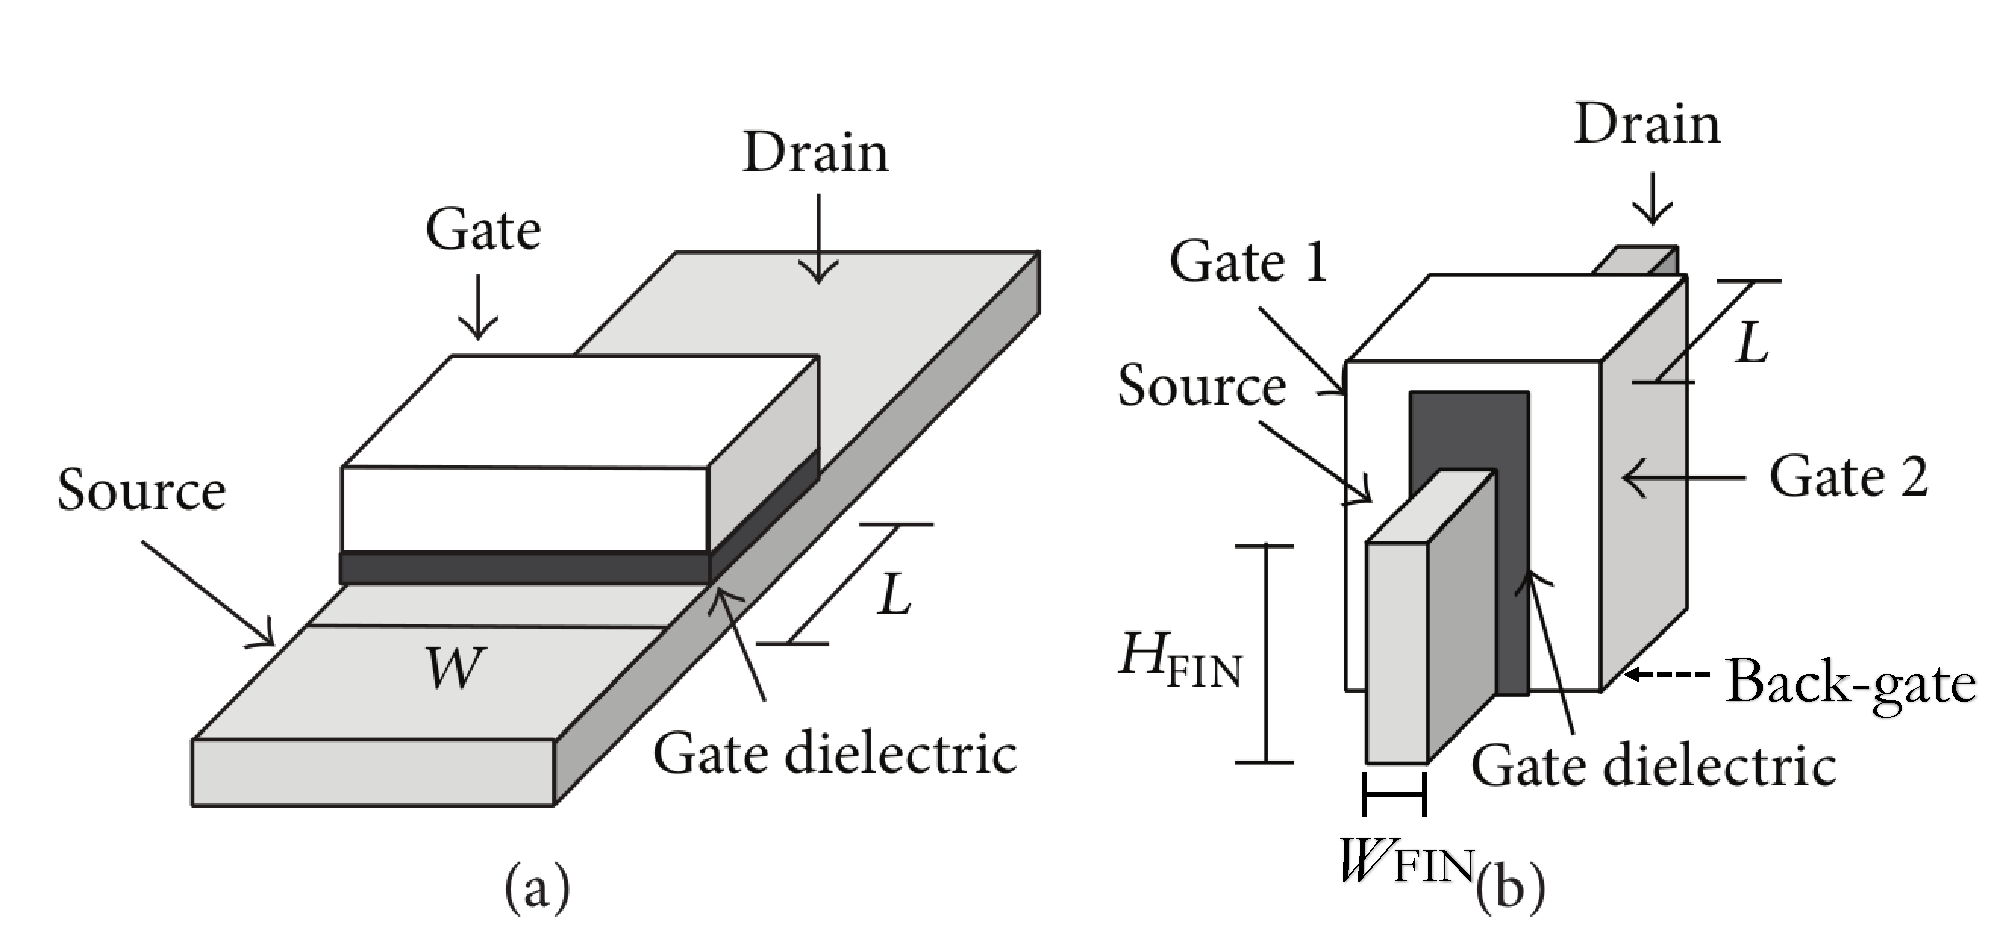
\includegraphics[width=\textwidth, trim={0 0cm 0 0cm},clip]{finfet.pdf}
\caption{Structural comparison between (a) planar MOSFET and (b) FinFET.}
\label{mosfetvsfinfet}
\legend{Source: \citet{bhattacharya2014finfets}}
\end{figure}

\begin{figure}[H]
\centering
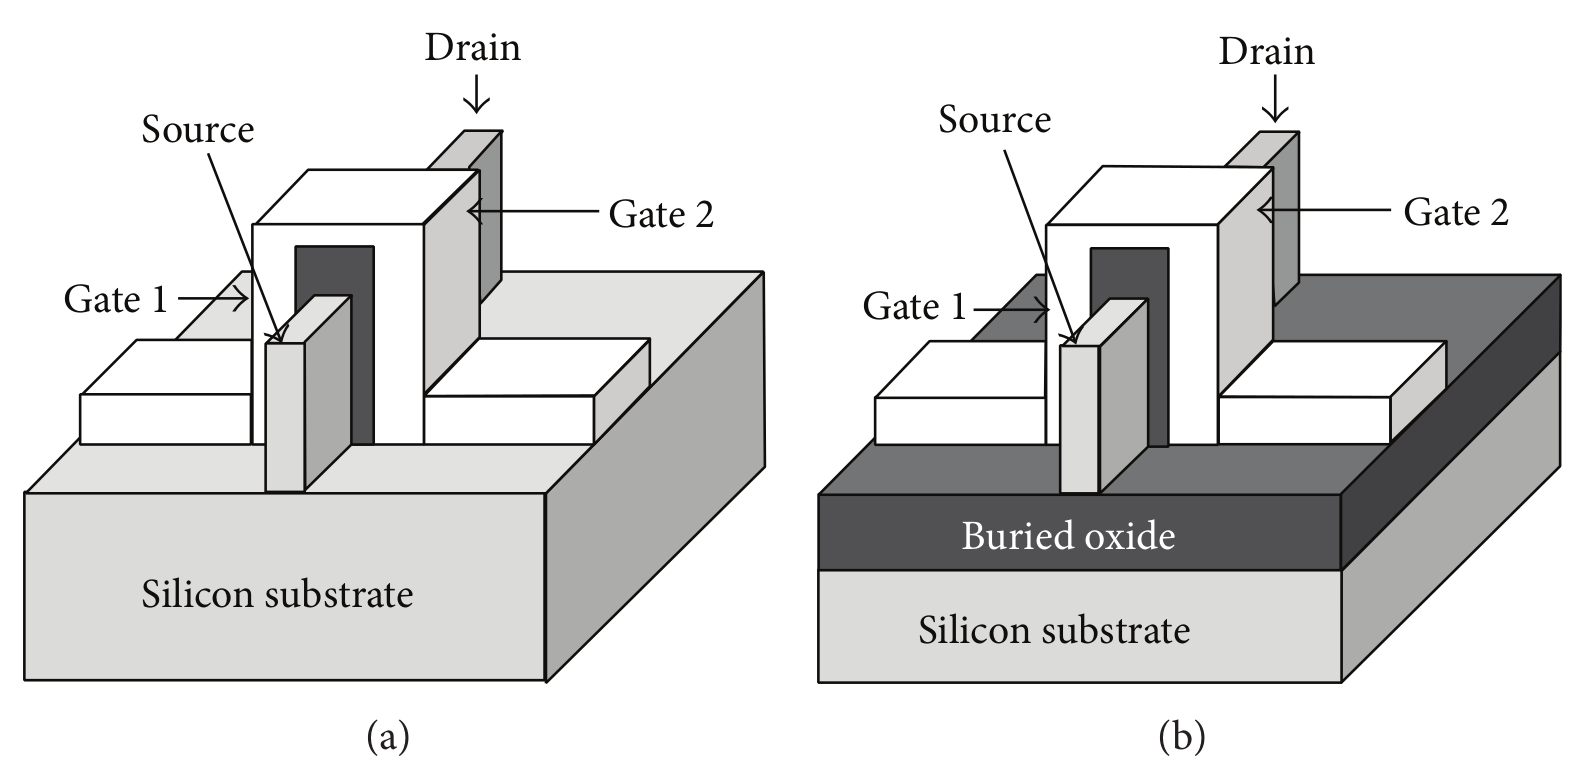
\includegraphics[width=\textwidth, trim={0 0cm 0 0cm},clip]{finfet2.png}
\caption{Structural comparison between (a) bulk and (b) SOI FinFETs.}
\label{bulkvssoi}
\legend{Source: \citet{bhattacharya2014finfets}}
\end{figure}

The channel being surrounded from three dimensions by the gate results in a superior control, reduced short-channel effect (SCE) and eliminated random dopant fluctuation (RDF) effect due to the fully depleted channel that causes less sensitivity to process variations \cite{taur2013fundamentals}. FinFETs also present relative immunity to gate line-edge roughness, a major source of variability in planar nanoscale FETs \cite{finfetchar1}. The disadvantage over MOSFETs is the harder manufacturing process due to difficulty in the lithography steps as it is increasingly difficult to print small patterns, the increased variability impact due to the further minituarization of dimensions, in comparison to MOSFET and more constly manufacturing process due to the need of techniques to address the manufacturing imprecision and, in the case of SOI FinFET, to change the CMOS substrate process to support a SOI substrate manufacturing process \cite{finfetchar1} \cite{finfetdis}.

Several works analyze the FinFET reliability. In \cite{FinFET01} it is shown, at 14/16nm fabricated bulk FinFET technology, that for high energy charged particles, the drive current is the dominant factor to the transient fault pulse width and cross-section. And low energy particles have a grater dependence on secondary transistor and circuit design factors (number of fins, transistor arrangement, etc). 

In \cite{FinFET02} the hot carrier injection (HCI) effect is analyzed in pass-gate FinFET transistors. The tests were executed using commercial FinFET technology showing a 50\% chance of errors due to HCI in pass-gate transistors. In \cite{FinFET03} a analysis of the sensitivity of double-gate and FinFET devices to process variations is shown. It is concluded that for 20nm FinFET devices large channel doping concentration is necessary to obtain suitable values of threshold voltage if heavily doped polysilicon gates are used. Due to the small volume of the channel the channel doping will bring unnacceptable V\textsc{th} fluctuations. Given that, heavily doped polysilicon may not be a viable choice with the work function adjustment being a better approach. 

In \cite{FinFET04} the modeling of the reliability degradation of a FinFET-based Static Random Access Memory (SRAM) is shown. It is concluded that the probability of failure due to Bias Temperature Instability (BTI) and Gate Oxide BreakDown (GOBD) is relatively lower in comparison to HCI-induced failures. They also shown the improvement of lifetime due to Error-Correcting Code (ECC) memory. In \cite{FINFET05} a investigation on reliability characteristics of NMOS and PMOS FinFETs is conducted. Based on fabricated FinFETs transistor with 17-27 nm width, it was shown that the life time of FinFET is very dependable of its dimensions. The predicted lifetime for a 50nm gate length NMOS FinFET was 133 years, for the first HCI event. While a 27nm fin-width PMOS FinFET showed 26.84 years of lifetime wich is reduced to 2.76 years when reducing its fin-width from 27 to 17 nm for a NBTI event, showing the huge reliability challenge introduced by technology scaling.

Given the majority of papers exploring the reliability factors and its effects but the few that actually study mitigation techniques, this paper aims to bring a layout level analysis of a novel technique for robustness improvement. There is no evaluation in the the literature of the impact of the ST technique at layout level as well as in FinFET technology.

\chapter{Variability Effects and Mitigation Techniques}

Standard CMOS devices have been optimized for high-speed and low-power consumption through its lifetime being the backbone of almost all modern digital circuits. The periodic process of technology scaling has resulted in faster and more energy efficient transistor than the previous generation. As channel lengths shrank below 50nm, the ratio of device size to atom-size becomes smaller, hence, a variable structure at the atomic scale has an increased effect on device behavior. There have been advances to reduce the loss of precision due to the manufacturing process. However, the intrinsic quantum-mechanical limitations cannot be overcome, with their impact increasing as the technology shrinks further \cite{asenov1999random}. 

Variability can occur in both spatial and temporal domains with deterministic and stochastic fluctuations \cite{walker2010optimizing}. In summary, variability consists of deviation of characteristics, internal or external, to the circuit, which can determine its operational features such as power and delay. These characteristics, or factors, as we addressed them for the rest of this work, can be divided into three types: 
 
Environmental Factors:  
Caused by temperature fluctuations and voltage drops. Voltage drops occurs due to abrupt changes in the switching activity, causing large current transients in the system, which can occur locally as well globally across the die \cite{nassif:08}. 
 
Reliability Factors: 
Related to the aging process of the circuit, it is introduced by negative bias temperature instability (NBTI), positive bias temperature instability (PBTI), electromigration, time dependent dielectric breakdown, gate oxide integrity, thermal cycling and hot carrier injection \cite{nassif:08}.
 
Physical Factors:
It is related to variations caused by the manufacturing process, due to imprecisions in litography stage, which results in deviations in the electrical parameters defining the behavior of active and passive devices. Those variations can be divided in three types of mechanisms: Systematic, they repeat over many chips or wafers. Design dependent, being particular to each circuit design. And Random, which depends on the random aspects of process manufacturing, as shown in Figure \ref{fig:Fig2} \cite{nassif:08}.

Additionally, the technology scaling and manufacturing tolerances are not correspondingly moving side by side. For instance, the pace at which the effective channel length is reduced is faster than the improvement of mask fabrication error and mask overlay control \cite{nassif:08} \cite{aghababa2009static}.

\begin{figure}[H]
\centering
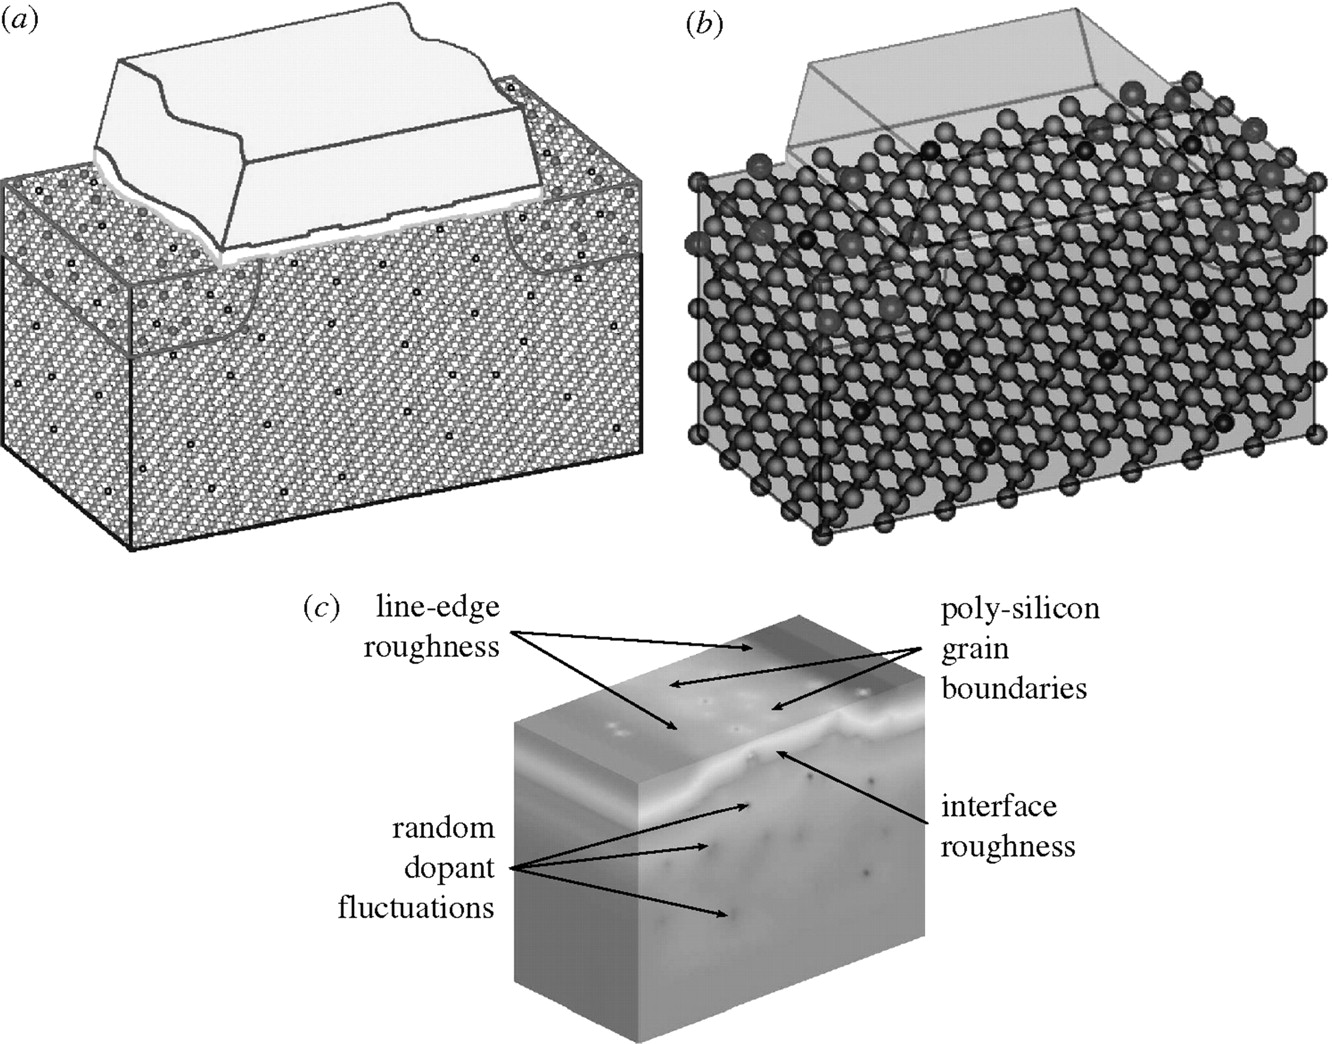
\includegraphics[width=\textwidth]{transistorVariability.jpg}
\caption{Transistor Variability}
\label{fig:Fig2}
\legend{Source: \citet{walker2010optimizing}}
\end{figure}

These three types of variabilities, in conjunction, may prevent circuits from meeting their performance and power goals. Table \ref{tab:02} demonstrates the design impact of performance and power due to different types of variability.

\begin{table}[H]
\centering
\caption{Design impact on performance and power due to different types of variability}
\label{tab:02}
\resizebox{\textwidth}{!}{%
\begin{tabular}{lcccc}
\hline
Property & Ease of measuring & Variability & Effects of Variability & Effect of missing specification \\ \hline
Performance & Medium & Medium: up to 60\% & L, W, R, C, Vth, \(\mu\) & Slower product, yield, timing error \\ \hline
Leakage Power & Easy & Large: up to 148\% & L, Vth, \(\mu\), tox & Shorter battery life, yield , heat \\ \hline
Dynamic Power & Difficult & Workload dependent & C,  \(\alpha\) & Shorter battery life, heat \\ \hline
\end{tabular}%
}
\legend{Source: \citet{rahimi2016variability}}
\end{table}

This work evaluates the effects caused by the physical variability. In FinFET, the physical variations are responsible for deviations in the device work function (WF), gate length (L\textsc{g}), fin height (H\textsc{fin}), fin thickness (T\textsc{si}) and parasitic resistances. It is shown in \cite{meinhardt2014impact} that work function fluctuation (WFF) is the main cause of threshold voltage (V\textsc{th}) variations. Alongside, in \cite{wang2011statistical} is shown the high correlation between the variability in the on (I\textsc{on}) and off (I\textsc{off}) currents and V\textsc{th} fluctuation in the presence of granularity of the metal gate. The main cause of WFF is due to its dependency over the orientation of its metal grains. In the real fabrication process, metal gate devices are generally produced using multiple types of metal with different work functions randomly aligned as depicted in Figure \ref{wff}. In the ideal fabrication process, metal gate devices have the gates manufactured with uniformly aligned metal and then, they have very low WFF deviation \cite{meinhardt2014impact}.

\begin{figure}[H]
\centering
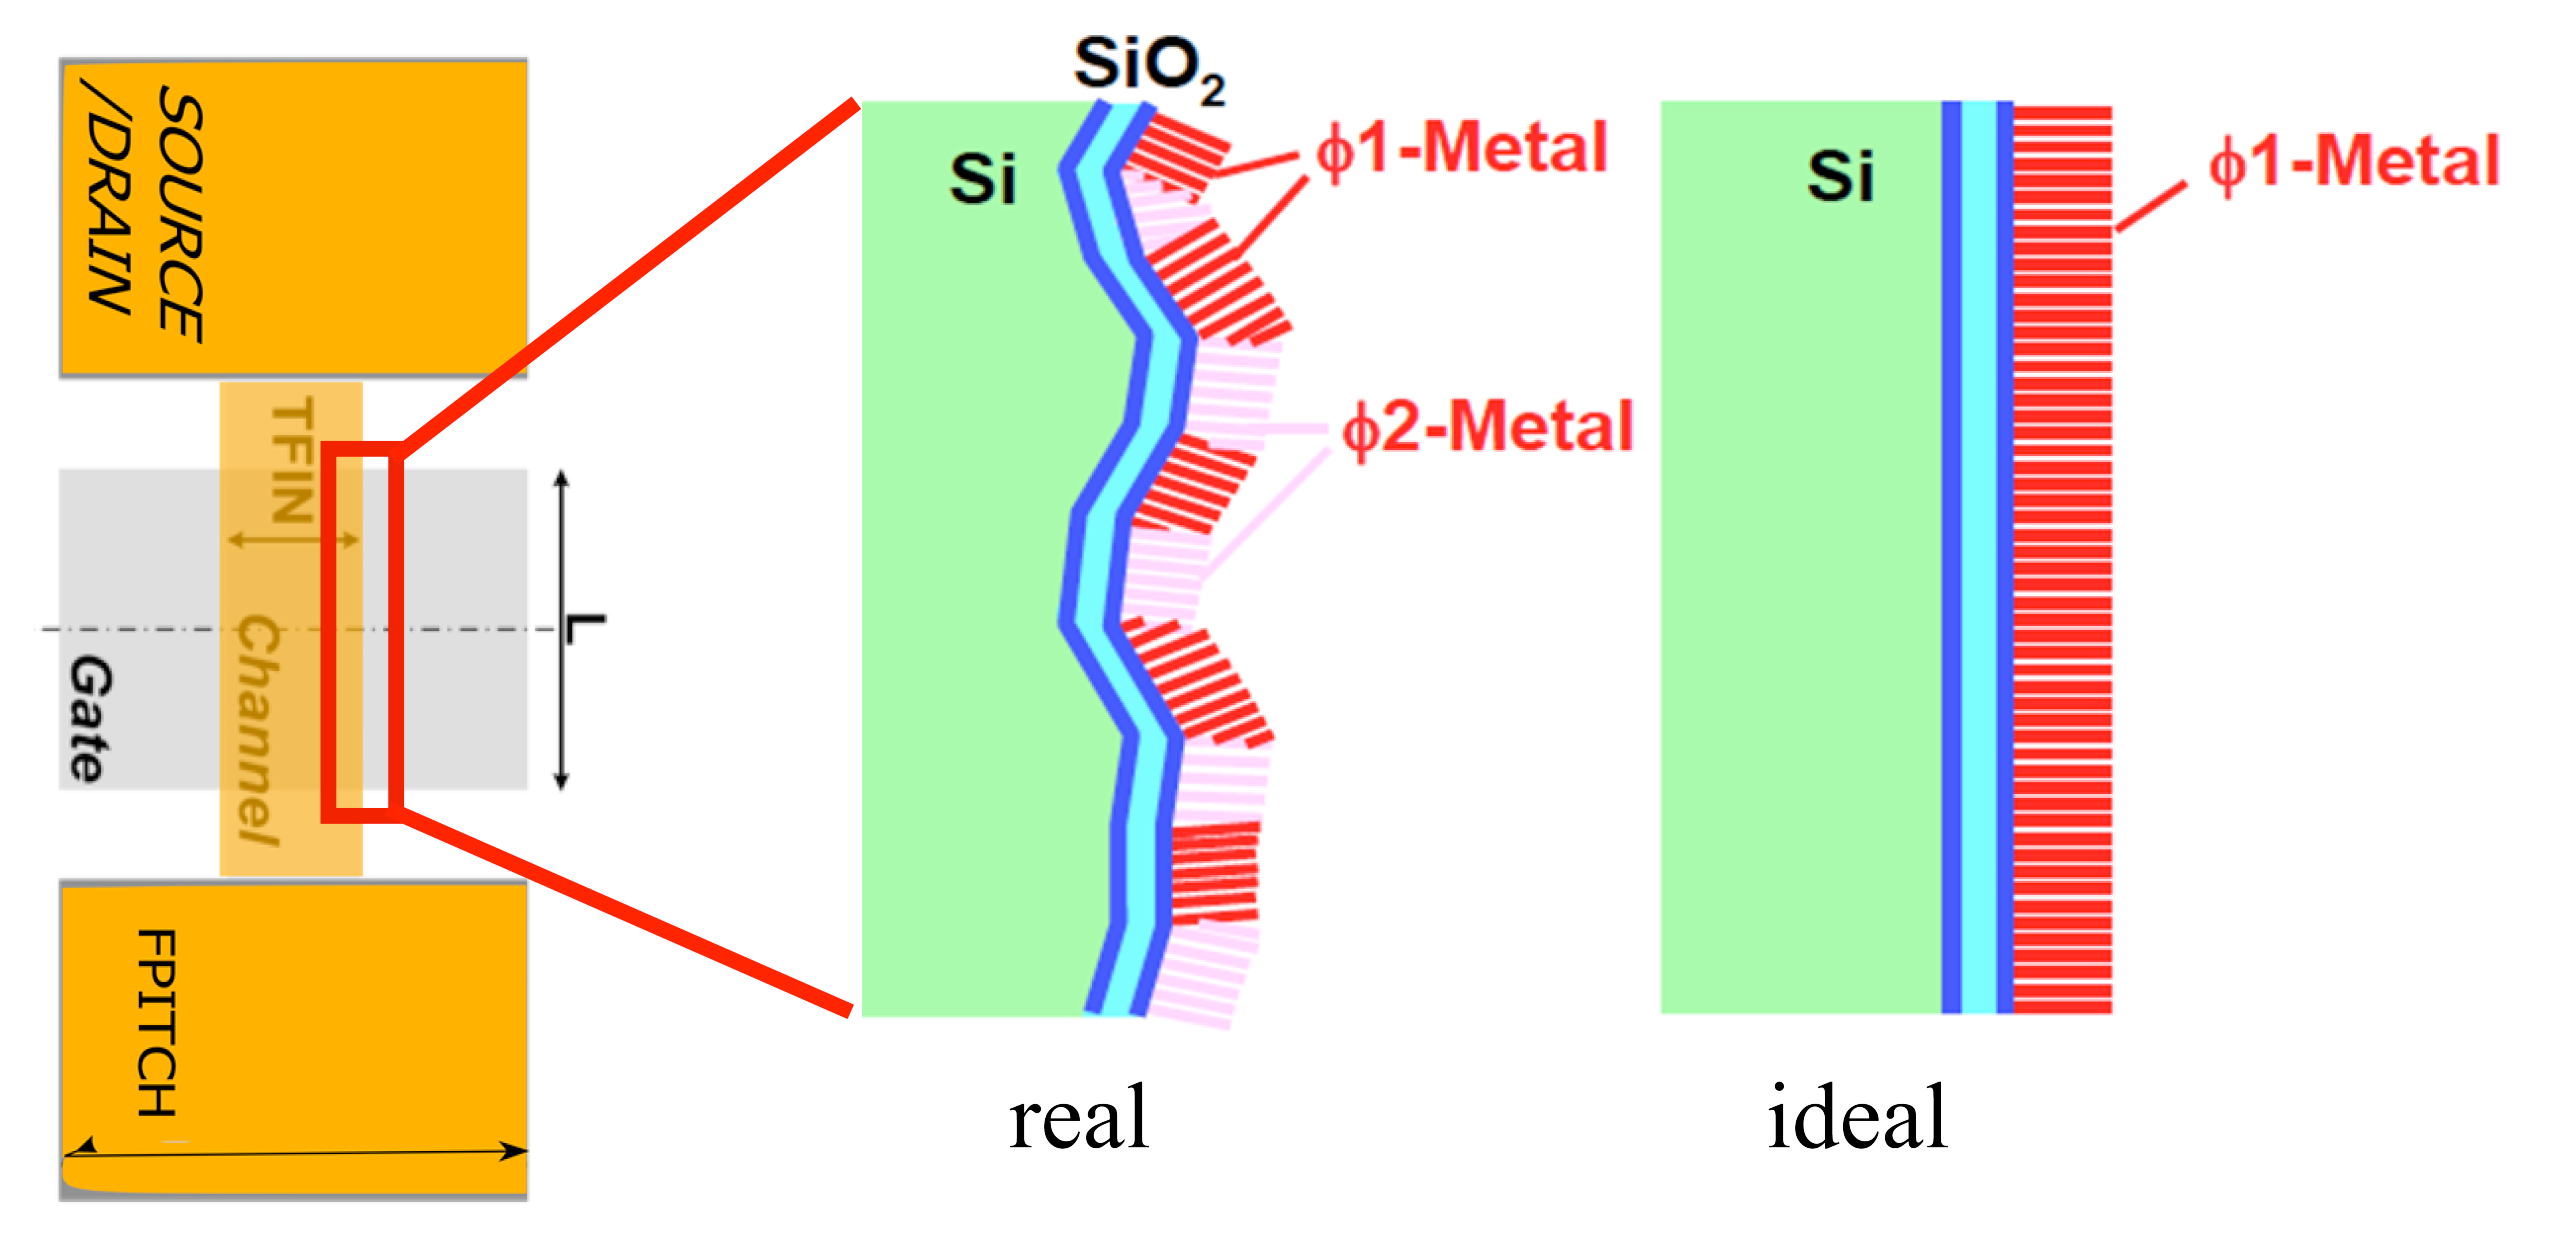
\includegraphics[width=\textwidth]{wff.png}
\caption{Metal gate fabrication ideal and real aspects.}
\label{wff}
\legend{Source: \citet{meinhardt2014impact}}
\end{figure}

\section{Related Works}

At circuit level there is multiple techniques to predict and prevent errors: Tuning CMOS knobs, circuit topology optimizations, self-timed circuits, temporal and logical error masking, relaxed retiming and graceful degradation, and inexact circuits. Although, there are few approaches to decrease the process variability at its core. It is due to the technology dependency present in this problem \cite{rahimi2016variability}.

It can be observed that many works try to indicate the most robust design for a given type of circuit. For example, in \cite{dokania2013investigation} twelve different Full Adder topologies are analyzed considering delay, power and Power-Delay-Product (PDP) variability. It is used a 16nm bulk CMOS technology node in SPICE simulations with Process, Voltage and Temperature (PVT) variability being considered and Monte Carlo simulations performed. The authors concluded that Cell A, CLRCL and Cell B full adders presented the best results for all three metrics (Delay, Power and PDP).

In \cite{ames2016investigating} the effects of PVT variability in different full adder designs are investigated. The simulations are performed in HSPICE with the bulk CMOS 32nm node technology. With Transmission Gate Full Adder (TGA) and Transmission Function Adder (TFA) architectures showing acceptable behavior under PVT variability with the lowest power consumption sensibility amongst the tested full adders - 11x smaller in comparison with Complementary Pass Transistor Logic (CPL) Full Adder.

In \cite{islam2011design} various popular 1-bit digital summing circuits functionality and robustness are analyzed in light of PVT variations with the best full adder being simulated in Carbon Nanotube Field Effect Transistor (CNFET) technology for comparison with the bulk CMOS version. The simulations are carried at the 22nm bulk CMOS and CNFET technology node in HSPICE. Its results show that the TGA has the strongest PVT variability robustness and its CNFET version provides over 3x, 1.14x and 1.1x less propagation delay, power dissipation and energy delay product (EDP) variations, respectively. This work does not consider the total power consumption of each full adder separately.

Some articles analyze the adoption of new technologies: \cite{guduri2015design} proposes a hybrid of bulk CMOS and CNFET Full Adder at 16nm in deep subthreshold operation region for ultralow-power applications simulated in SPICE which showed some improvement over its bulk CMOS Full Adder counterpart achieving 5\% and 1\% improvement in power, power-delay and energy-delay products and their variability, respectively.  

In \cite{islam2011variability} a new subthreshold-FinFET Full Adder is proposed and compared over multiple full adders showing huge metric improvements provided by the FinFET technology up to 2.22x improvement in power variability. It was simulated in 32nm predictive technology model on HSPICE. 

It is notable that none of these works consider a layout approach for its simulations and do not address any novel general technique which can be applied to a range of different types of circuits. Although, some works introduce novel designs.

\cite{federspiel201228nm} presents reliability comparison between 28nm bulk CMOS and Fully Depleted Silicon On Insulator (FDSOI) technologies at layout level, with FDSOI showing 32\% improved performance, 40\% reduced power consumption and improved matching, with its intrinsic reliability behavior similar to 28nm bulk at the device level. \cite{alioto2007delay} presents a study about the delay variability caused by supply variations in the TGA. The experiments were performed at 90nm and 180nm bulk CMOS Technology in Spectre at layout level. It showed that lower supply voltages bring more delay variability to the circuit with the TGA presenting worse results 15\% (25\%) for the 90 nm (180 nm) in comparison to static logic.

Some works focus on evaluating techniques: In \cite{zimpeck2016finfet} three dimensioning methods are applied on multiple circuits and their impact on variability robustness is analyzed. The simulations were performed considering a 14nm FinFET technology using HSPICE tool. The authors concluded that the Optimized Transistor Sizing (OTS) technique has the best ratio between nominal PDP and PDP under process variability.

\cite{ahmadi2017hybrid} introduces a new technique to improve the performance of digital circuits in the presence of variations. It consists of a hybrid of two former methods to prevent errors due to delay variations. The simulations were performed with a 45nm predictive technology using HSPICE and applied on ITC’99 and ISCAS’89 benchmarks circuits. The results show that this hybrid technique can tolerate process variations up to 27.3\% better than state-of-the-art techniques.

Among these works there is \cite{dokania2015circuit} on which a novel technique based on the replacement of Full Adder’s internal inverters with low voltage Schmitt Triggers for PVT variability robustness improvement is originally introduced and applied on seven different full adder designs. The simulations were performed using the 16nm bulk CMOS predictive technology model in SPICE. It presented significant variability improvement up to 4.8x in PDP. Although, the improvements occur at the cost of an increase in the area and power dissipation of each design.  

Alongside, in \cite{samuel2016} the ST technique is applied on four Full Adders. It presented promising results regarding the power deviation due to the process variability with a decrease up to 79\% with a drawback of a significant increase in average energy consumption. The simulations were performed with the 16nm technology predictive technology model in NGSPICE. 

Schmitt triggers are commonly used as internal circuits on systems to provide enhanced noise tolerance and robustness against random variations in the input waveforms. On a typical input (non-Schmitt trigger), its binary value will switch at the same point on the rising and falling edges. With a slow rising edge, the input will change near the threshold point. When the switching occurs, it will require current from the supply source. With current being pushed from the supply, it can cause a voltage drop across the circuit causing a shift in the threshold voltage. 

If the threshold shifts, it will cross the input causing it to switch again. It can go indefinitely causing oscillation. The same thing can happen if there is noise on the input. Schmitt Triggers are applied in these cases to filter noise introducing superior and inferior threshold voltages, as shown in Figure \ref{fig:Fig3}.c. The difference between the thresholds is called Hysteresis \cite{WinNT}, its curve is shown at \ref{fig:Fig3}.a. According to the Schmitt Trigger behavior, it can mitigate the influence of variations in the inputs product of PVT variability. In figure \ref{fig:Fig3}.c is shown a classical CMOS Schmitt Trigger design. 

\begin{figure}[H]
\centering
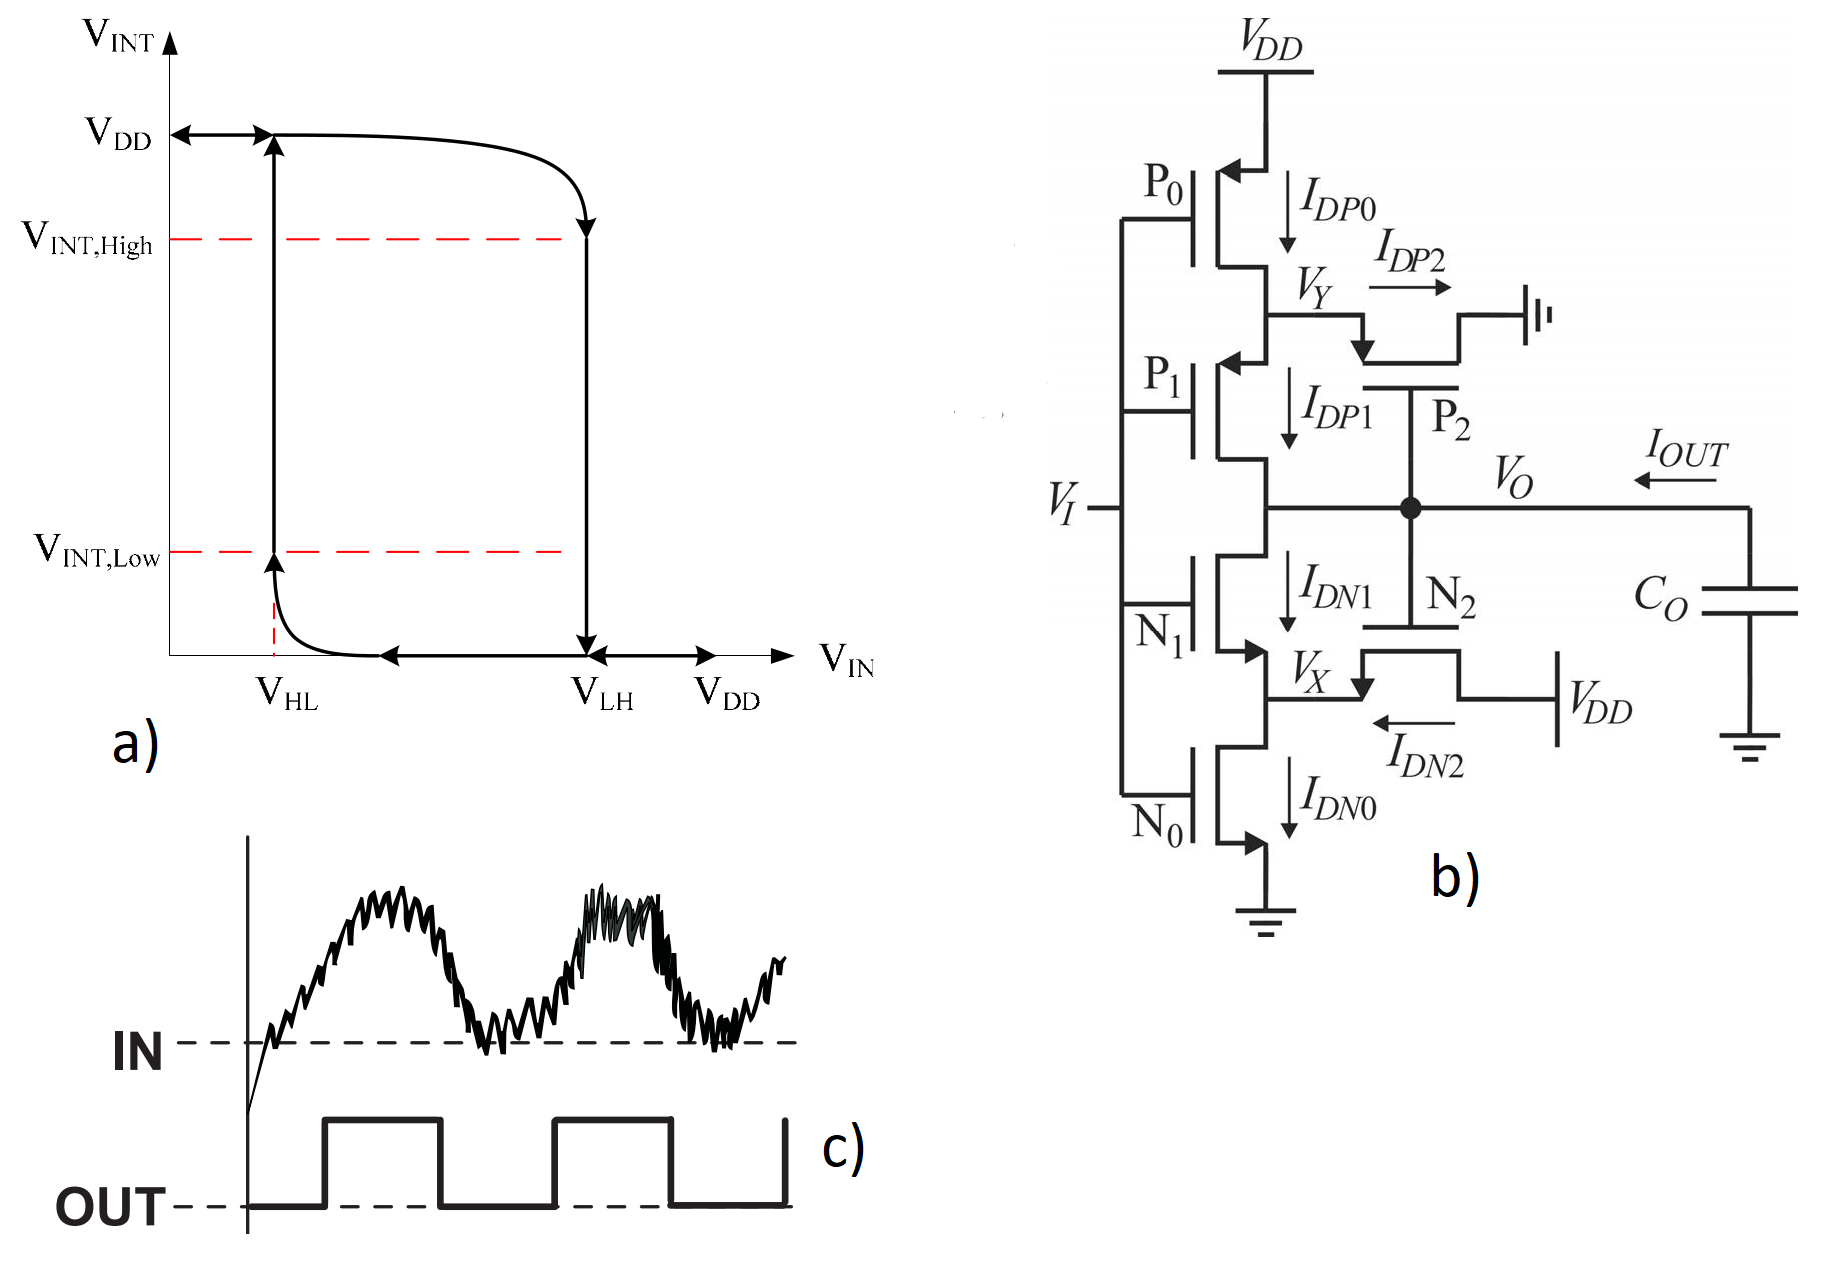
\includegraphics[width=0.8\textwidth]{Hysteresis.png}
\caption{a) General ST hysteresis curve b) Classical CMOS ST Topology c) Typical signal filtering with ST.}
\label{fig:Fig3}
\legend{Source: \citet{WinNT}}
\end{figure}

This technique is tested in several works: In \cite{ahmad2016single} it is presented a novel Schmitt-trigger-based single-ended 11 Transistor SRAM cell. It analyses its performance against seven different SRAM topologies. The novel cell showed the least energy consumption per operation with the smallest leakage power and a 6.9x higher Ion/Ioff ratio. Further PVT variability simulations confirmed the robustness of the design regarding read and write operation. The simulations were carried in 22nm predictive technology using HSPICE.

\cite{moghaddam2017design} presents a Schmitt trigger (ST) buffer using CNFET. It was evaluated against other two buffers and showed, on average, 68\% higher critical charge and 53\% lower energy consumption and a huge gain considering PVT variability robustness. The simulations were carried in 16nm Stanford CNFET model using HSPICE.

\chapter{Methodology}

For the experiments, there were considered four different types of Full Adders topologies to evaluate their robustness to process variability with their internal inverters replaced by Schmitt Triggers. The Full Adders listed below have been chosen due to their promising results in related works \cite{ames2016investigating} \cite{dokania2015circuit} \cite{dokania2013investigation}:

\begin{enumerate}
    \item Complementary MOSFET Adder (CMOS)
    \item Transmission Gate Adder (TGA)
    \item Transmission Function Adder (TFA)
    \item Hybrid Full Adder
\end{enumerate}

The CMOS Full Adder is considered the most traditional Full Adder topology containing 28 Transistors arranged in a pull-up and pull-down networks, which are logically complementary. It has a full voltage swing and buffered Sum and Cout signal and the advantages of good conductibility and robustness when working with novel technologies and low voltages. However, it has high capacitance because each input is connected to the gate of at least a p-channel metal-oxide-semiconductor (PMOS) and n-channel metal-oxide-semiconductor (NMOS) device additionally, it shows the impact of the pull-up network that makes the circuit slower due to the low mobility of its holes \cite{beckett2002fine} \cite{devadas2017design} \cite{islam2011design}. 

Transmission Gate Full Adder \cite{weste1985principles} contains 16 transistors, and is a high speed and low power design. However, shows low driving capability which may be unacceptable in some cases where there is a long chain of full adders due to the increase in delay \cite{islam2011design}. The Transmission Function Adder is based on transmission gates as well, containing 20 transistors, working satisfactorily with low voltages but losing performance when cascaded due to the lack of supply/ground contacts and, consequently, driving capability \cite{navi2009novel}. Both TFA and TGA generate the XOR function (H = A XOR B) followed by an inverter which produces the XNOR function (H’). H and H’ are used to control the transmission gates generating the Sum and Cout outputs. The inverter generates delay between H and H’, which will cause the transmission gates to behave as pass transistors, that may introduce glitches and consequently, increase the power consumption of these cells. Additionally, TGA contains three inverters, one more than TFA. The inverters switching introduce more short-circuit power \cite{shams2000novel}.

Inspired by CMOS and CPL Full Adders architectures, the Hybrid Full Adder \cite{navi2009novel} contains 26 transistors, with the main advantage of a high output signal and low power properties. Although, the design shows high input capacitance for specific input vectors. The Full Adder designs are shown in Figure \ref{fig:Fig5}.

\begin{figure}[H]
\centering
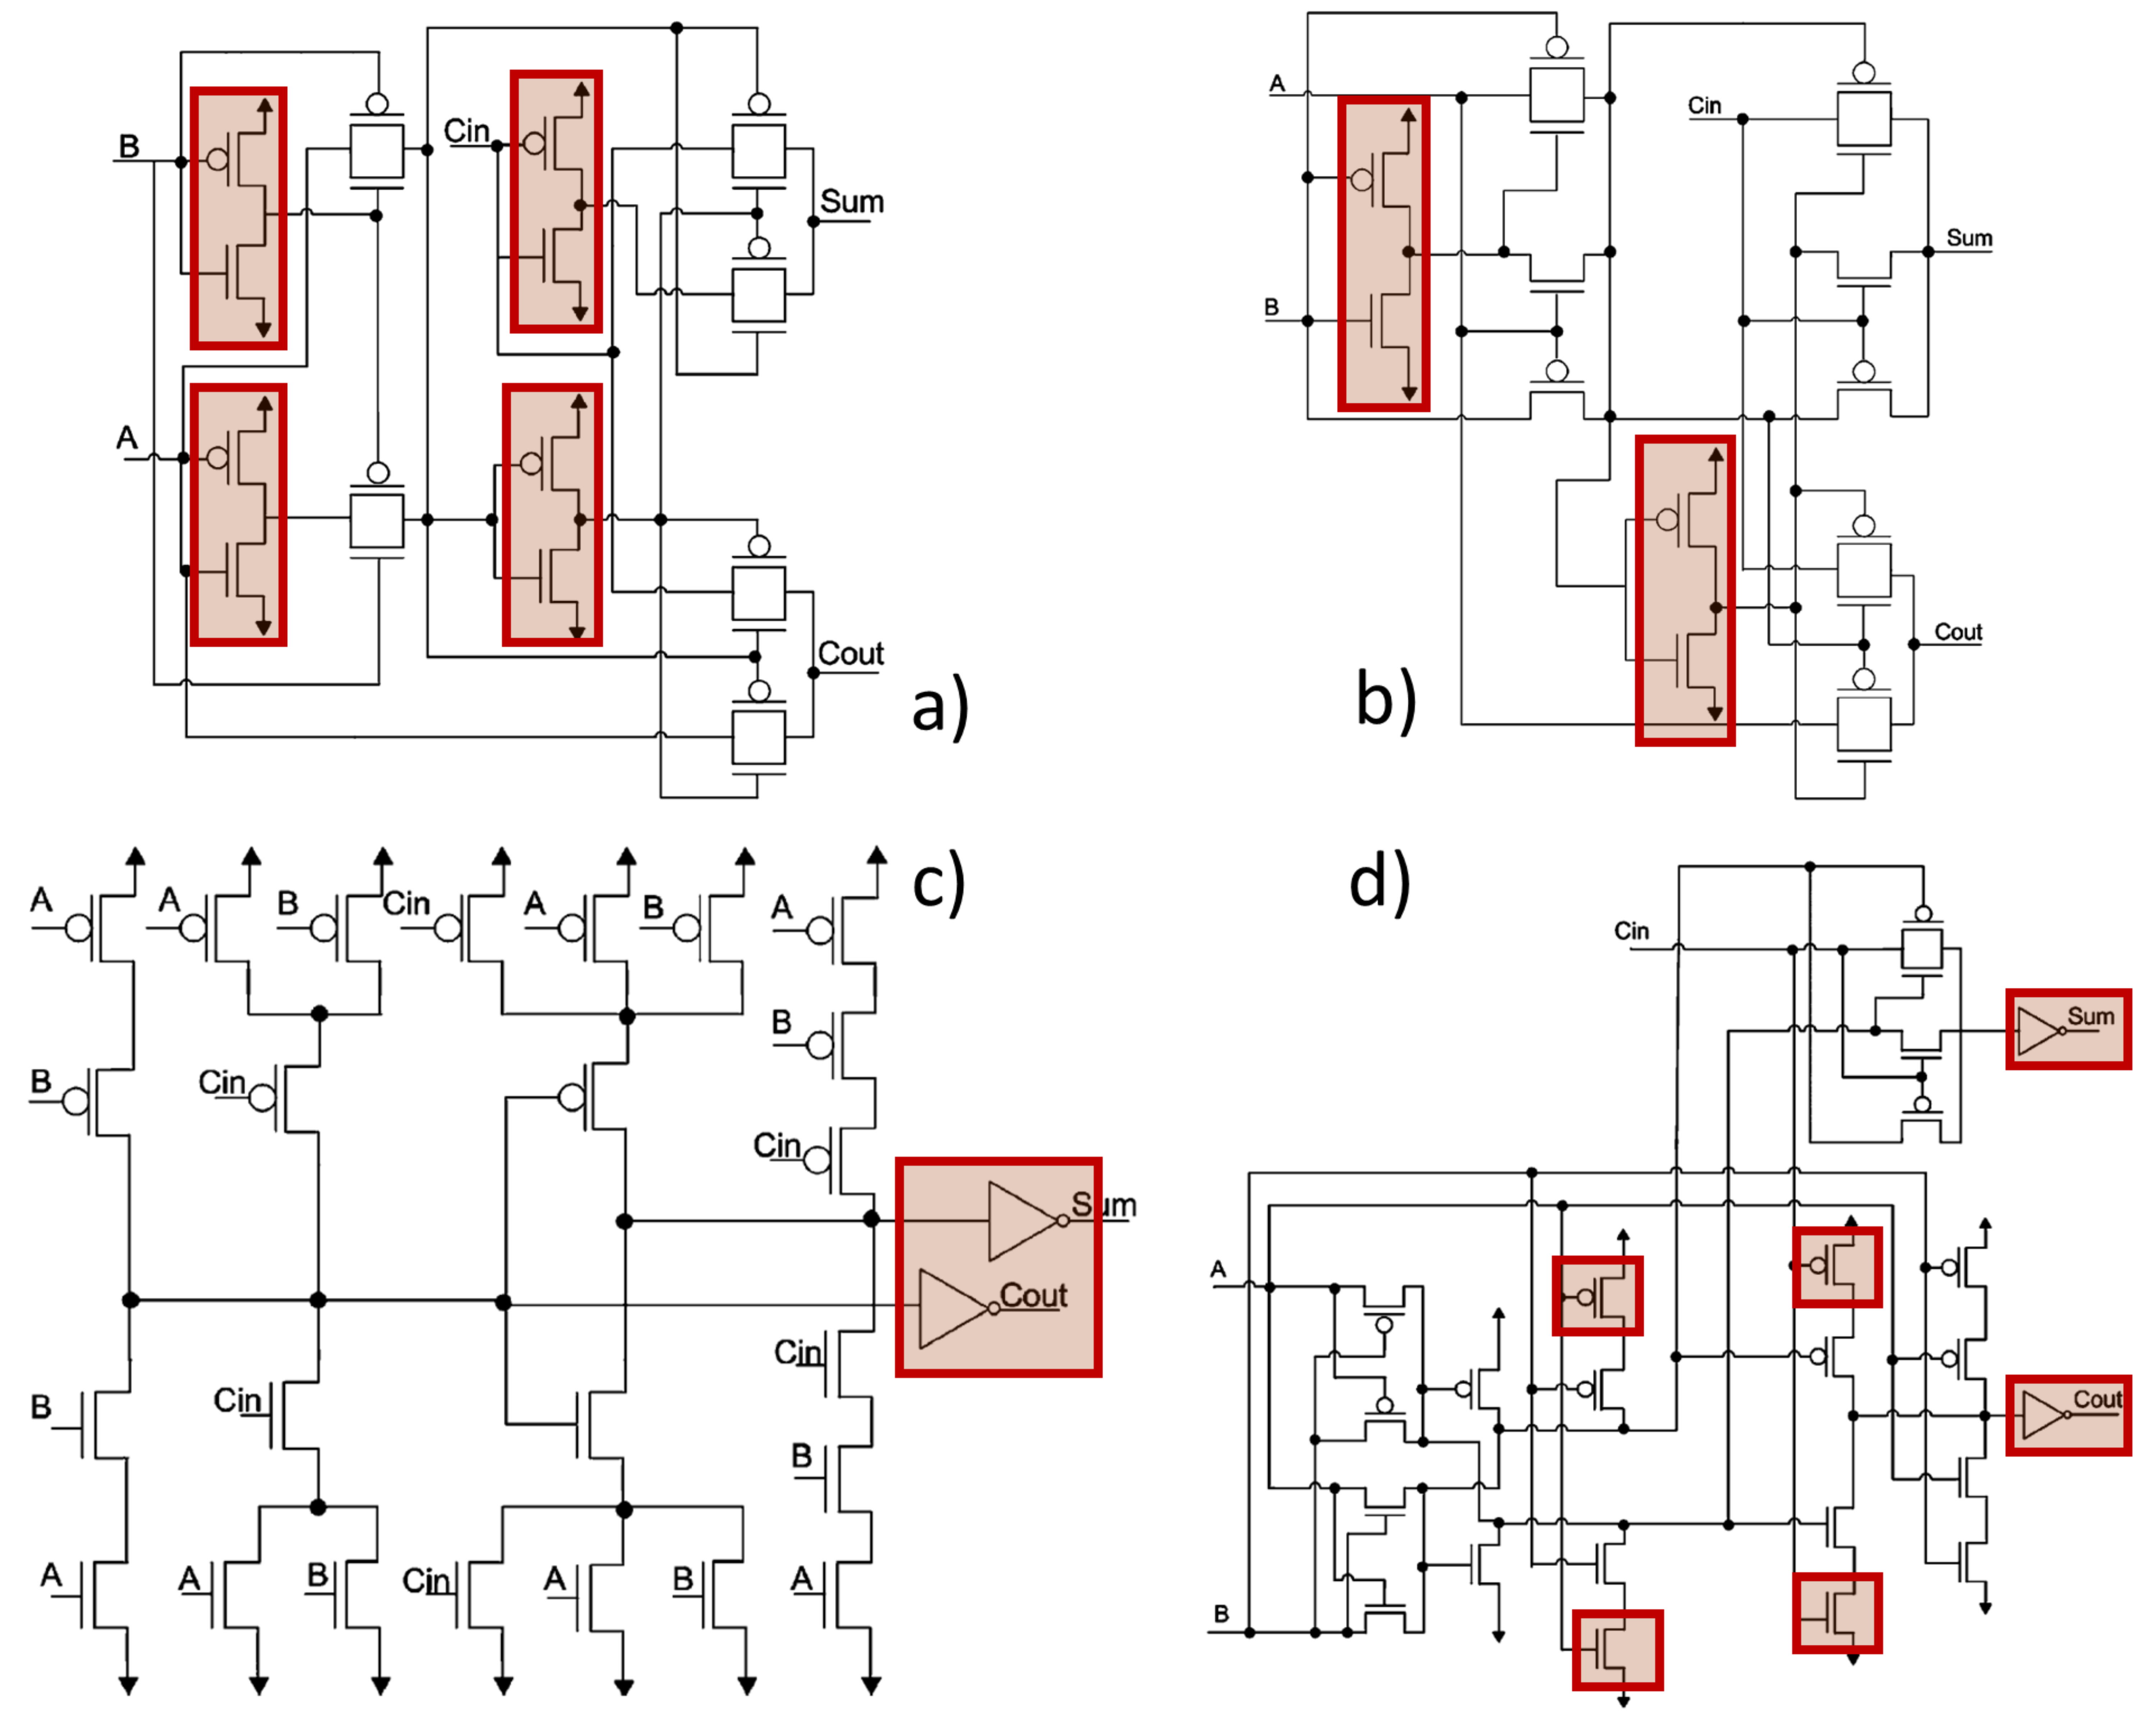
\includegraphics[width=1\textwidth]{FAs.png}
\caption{Full Adders with internal inverters to be replaced highlighted.}
\label{fig:Fig5}
\legend{Transmission Function Adder (a), Transmission Gate Adder (b), Mirror CMOS Adder (c) and Hybrid Full Adder (d).
Source: \citet{samuel2016}}
\end{figure}

A variety of CMOS Schmitt Trigger designs have been proposed and implemented over the years, with the conventional 6T-CMOS Schmitt Trigger proposed in \cite{doki1984cmos} exhibiting the wanted characteristics of different high-to-low and low-to-high transition threshold voltages, giving rise to hysteresis. The ST inverter circuit used in this work was inspired by \cite{zhang2003low} and modified in \cite{dokania2015circuit} to achieve the desired inverting characteristic, as shown in Figure \ref{fig:sub1}. It is designed for operation at a supply voltage of 0.4V in order to achieve low power consumption, and consists of the junction of two inverters where the output from the second one will be the bulk for the first one.  

In this design a dynamic body-bias technique is applied through a feedback mechanism to a standard CMOS inverter circuit, thus allowing a change in the threshold voltages of two MOSFETs, implying a change in the switching voltage. 

\begin{figure}[H]
\centering
\begin{subfigure}{.5\textwidth}
  \centering
  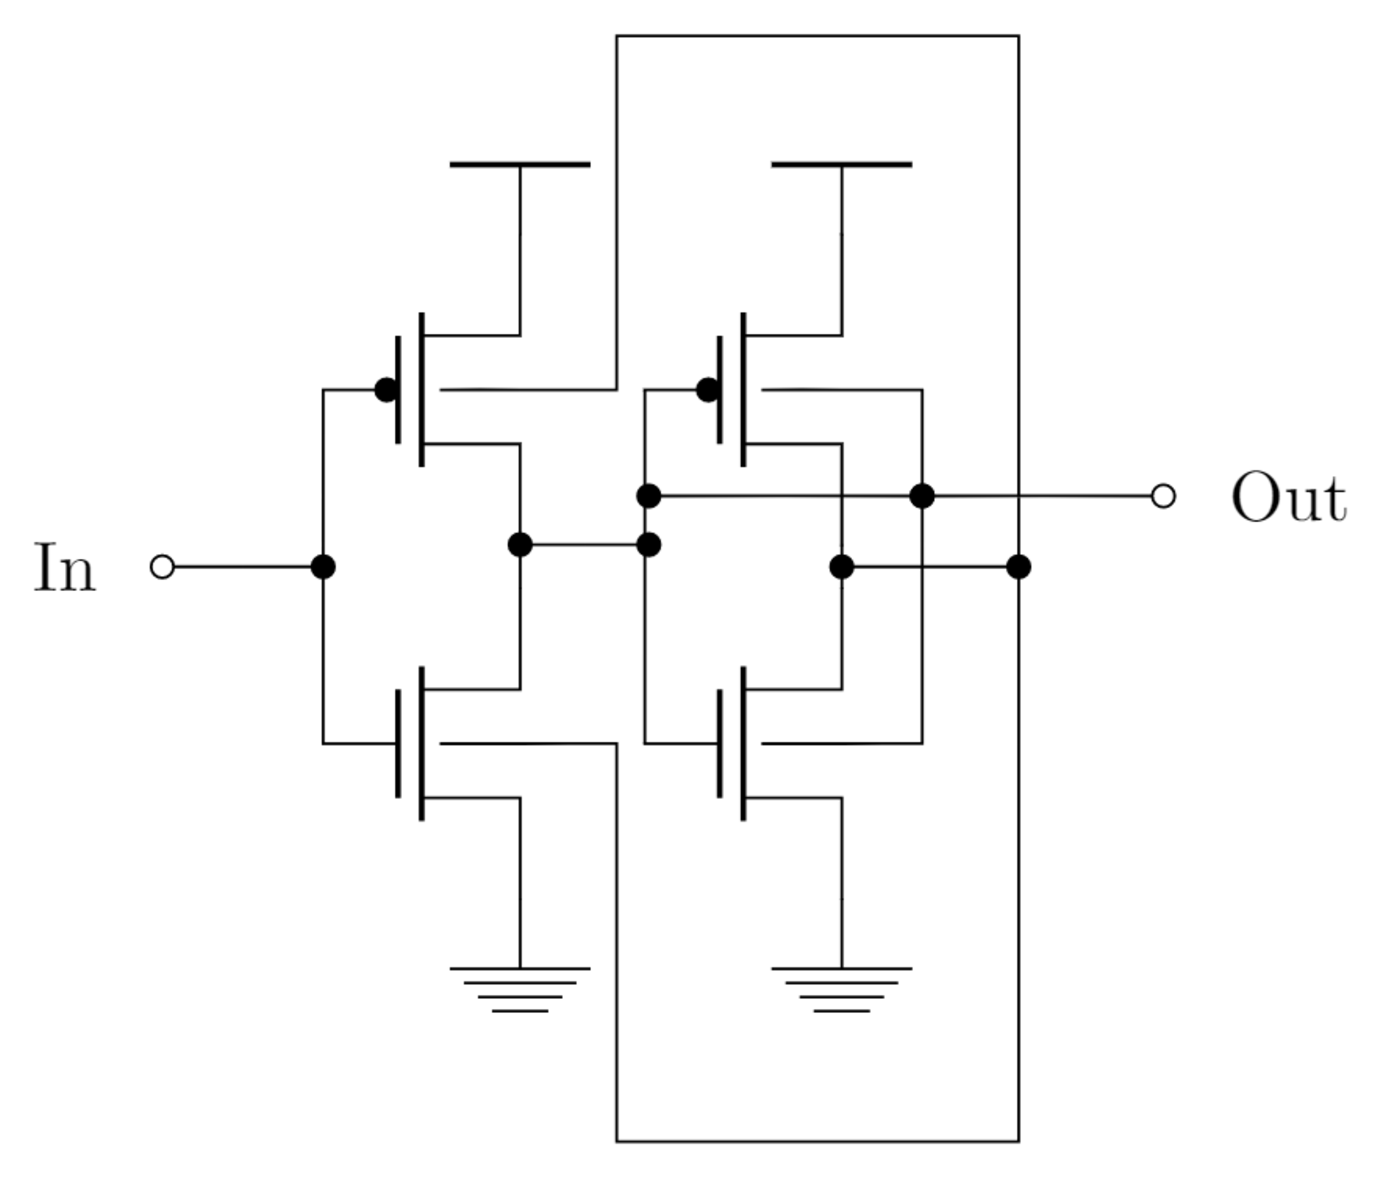
\includegraphics[width=.8\linewidth]{STOriginal.eps}
  \caption{ST Inverter from \citet{dokania2015circuit}}
  \label{fig:sub1}
\end{subfigure}%
\begin{subfigure}{.5\textwidth}
  \centering
  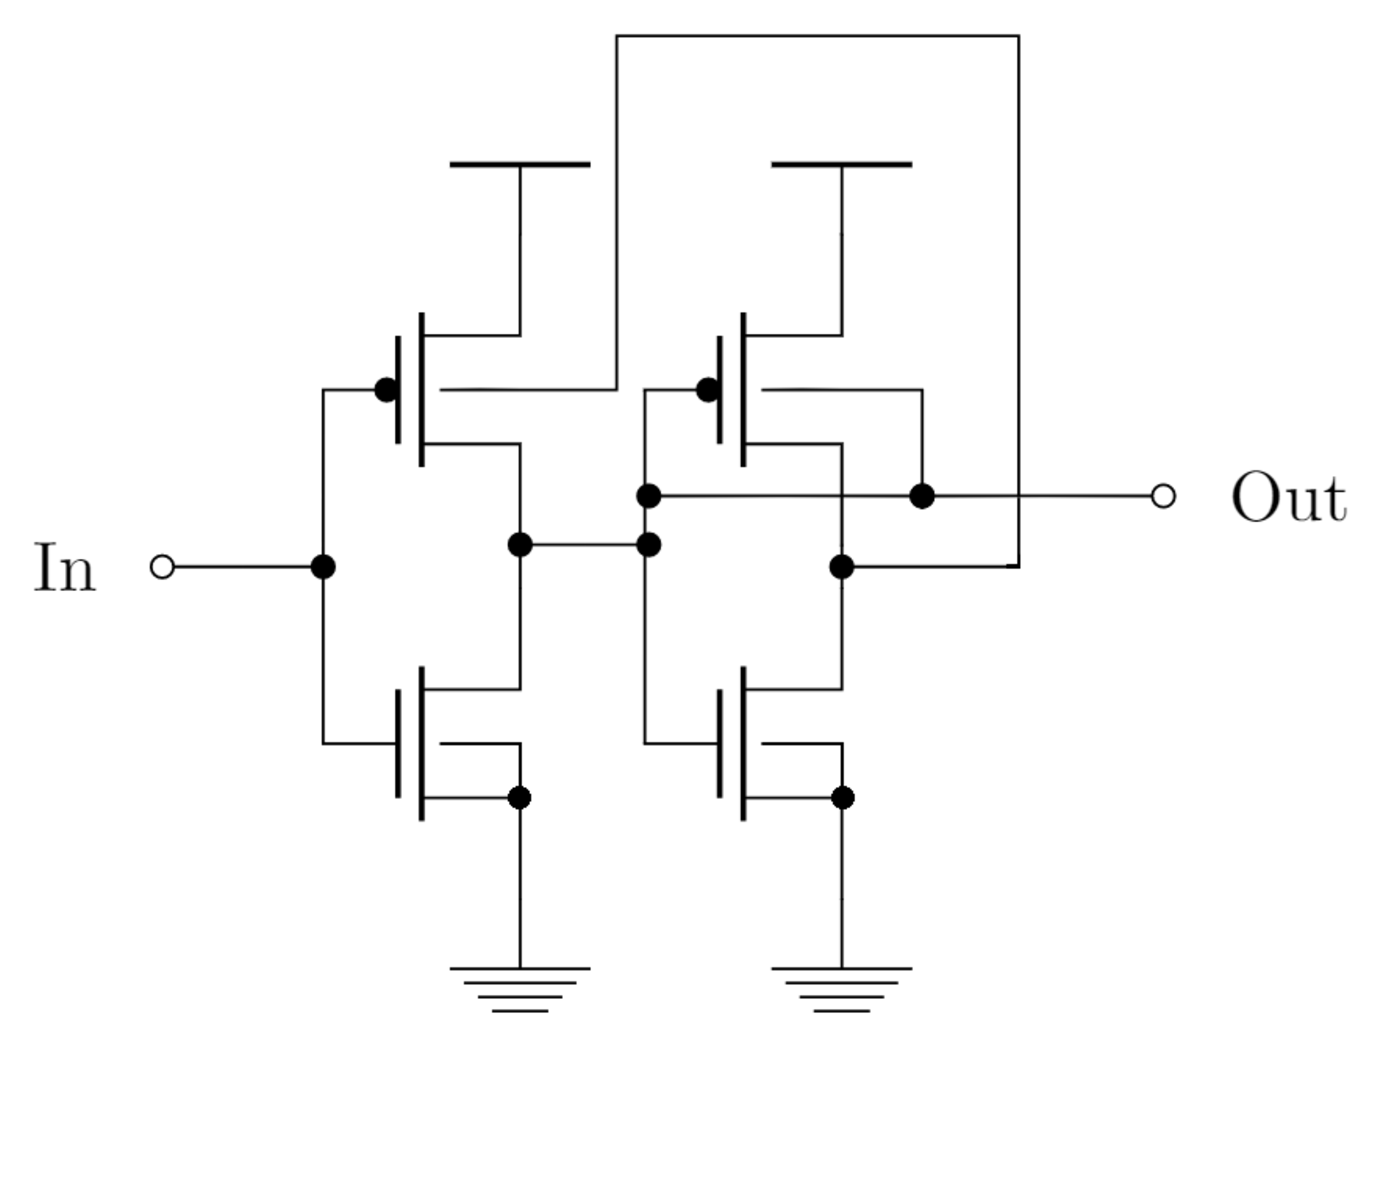
\includegraphics[width=.8\linewidth]{STcorrigido.eps}
  \caption{Modified ST Inverter applied in this work. Source: from author.}
  \label{fig:sub2}
\end{subfigure}
\caption{Original and modified STs side-by-side}
\label{fig:test}
\end{figure}

The project was divided into two main steps: The layouts design and the electrical simulations. Before the layouts design the Full Adders were chosen, based on \cite{dokania2015circuit} and the trasistor were sized (it was chosen 3 fins for each transistor). At Layout Design, each Full Adder schematic, symbol and Layout was designed. After finishing the layout design, each layout passed through validation which consisted from a Design Rule Checking (DRC) to detect if the layout obbeys the technology geometry restrictions and layer rules, Layout Versus Schematic (LVS) where layout and schematic are compared to detect if they are equals (same nodes and nets) and a Behavior test. After validation the layout netlist is generated with parasitics extracted. And, finally, the netlist is instantiated in a spice file with the technology WF variation inserted to simulate process variability. The design flow is shown at Figure \ref{DesignFlow}. In the end there was chosen 4 Full Adders. Each one was designed with and without the ST technique resulting in 8 layouts.

\begin{figure}[H]
\centering
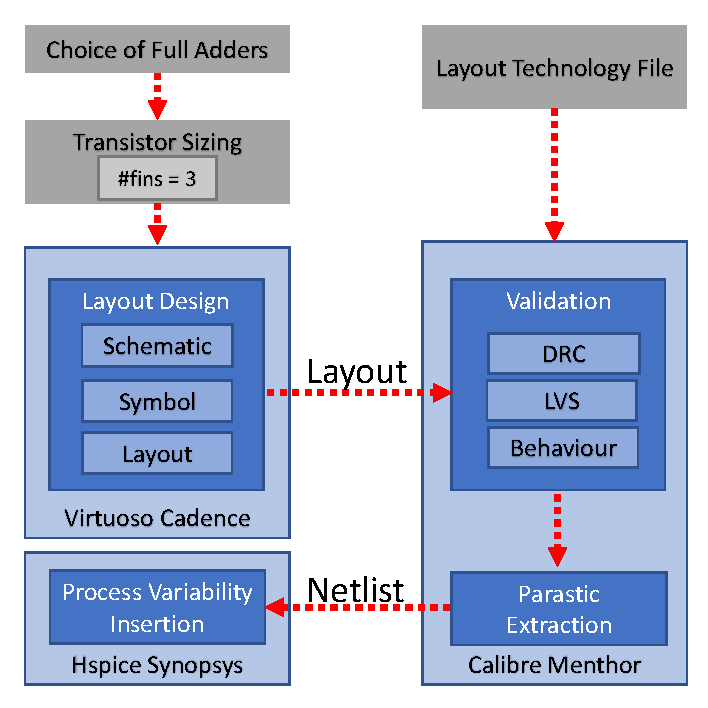
\includegraphics[width=0.8\textwidth]{DesignFlow.pdf}
\caption{Design flow of the experiments.}
\label{DesignFlow}
\legend{Source: from author.}
\end{figure}

\section{Layout Design}

All Full Adders layouts were designed using the Virtuoso Electronic Design Automation (EDA) tool from Cadence\textregistered{} with the process design kit (PDK) of 7-nm FinFET or Arizona State Predictive PDK (ASAP7) from the Arizona State University in partnership with ARM \cite{clark2016asap7}. It is the only available 7nm PDK for academic use, resulting in a very realistic estimative. This PDK was chosen due to realistic design conjecture regarding the current design competencies. Due to limitations of ASAP7 technology, it is not possible to connect the NMOS bulks separately due to the shared substrate. Given that, the Schmitt Trigger behavior is preserved with only minor changes between charging and discharging delays due to the difference between PMOS and NMOS threshold voltages. The ST applied in this work is shown at Figure \ref{fig:sub2}.

The main PDK rules and lithography assumptions considered in this work are shown in Table \ref{layers}. To exemplify the PDK layers, the traditional CMOS Full Adder layout is shown in Fig. \ref{fig:layers}. For all layouts it was used a dense 7.5 M2 (Metal 2) track cell, baseline resulting in a 270nm cell height. This corresponds to three fins for each transistor as shown in Figure \ref{th}. To make the back-gate connections it is necessary a TAP-Cell. It is responsible to connect the NMOS and PMOS back-gates to supply/ground, respectively, being possible to connect the PMOS back-gates to another node. It is a PDK restriction needed for the proper function of the circuit. Its layout has a length of 108nm resulting in an area of 0.02916 $\(\mu\)m^{2}$ as shown in Figure \ref{tap}.

\begin{table}[H]
\centering
\caption{Key layer lithography assumptions, widths and pitches}
\label{layers}
\begin{tabular}{lccc}
\hline
\multicolumn{1}{c}{\textbf{Layer}} & \textbf{Lithography} & \textbf{Width/drawn (nm)} & \textbf{Pitch (nm)} \\ \hline
\textbf{Fin}                         & SAQP                 & 6.5/7                     & 27                  \\ \hline
\textbf{Active (horizontal)}         & EUV                  & 54/16                     & 108                 \\ \hline
\textbf{Gate}                        & SADP                 & 21/20                     & 54                  \\ \hline
\textbf{SDT/LISD}                    & EUV                  & 25/24                     & 54                  \\ \hline
\textbf{LIG}                         & EUV                  & 16/16                     & 54                  \\ \hline
\textbf{VIA0-VIA3}                   & EUV                  & 18/18                     & 25                  \\ \hline
\textbf{M1-M3}                       & EUV                  & 18/18                     & 36                  \\ \hline
\end{tabular}
\legend{Source: \citet{clark2016asap7}}
\end{table}

\begin{figure}[H]
\centering
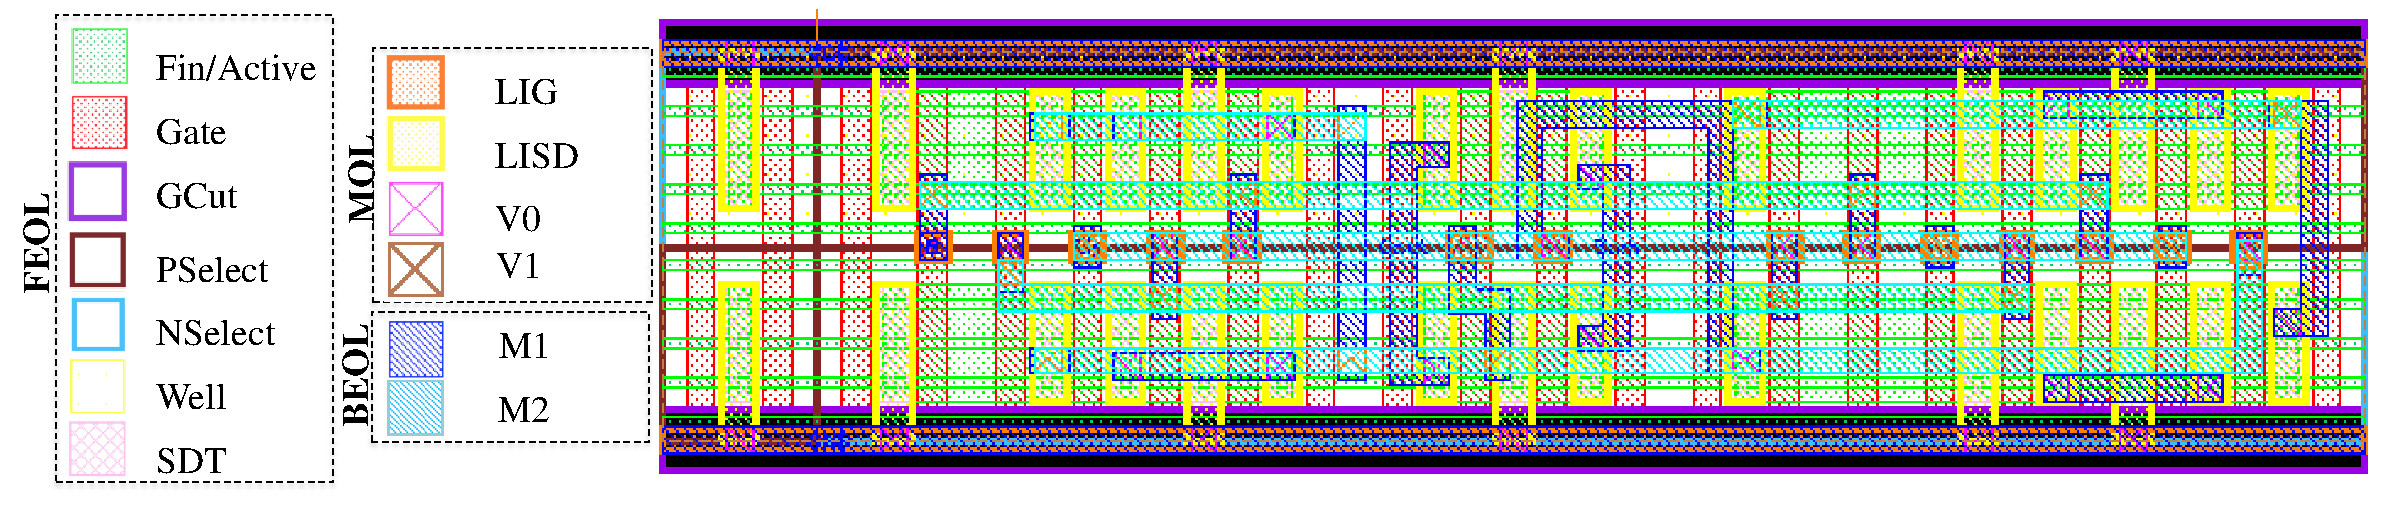
\includegraphics[width=\textwidth]{Layers.pdf}
\caption{Technology layers and original Mirror CMOS Layout}
\label{fig:layers}
\legend{Source: from author.}
\end{figure}

\begin{figure}[H]
\centering
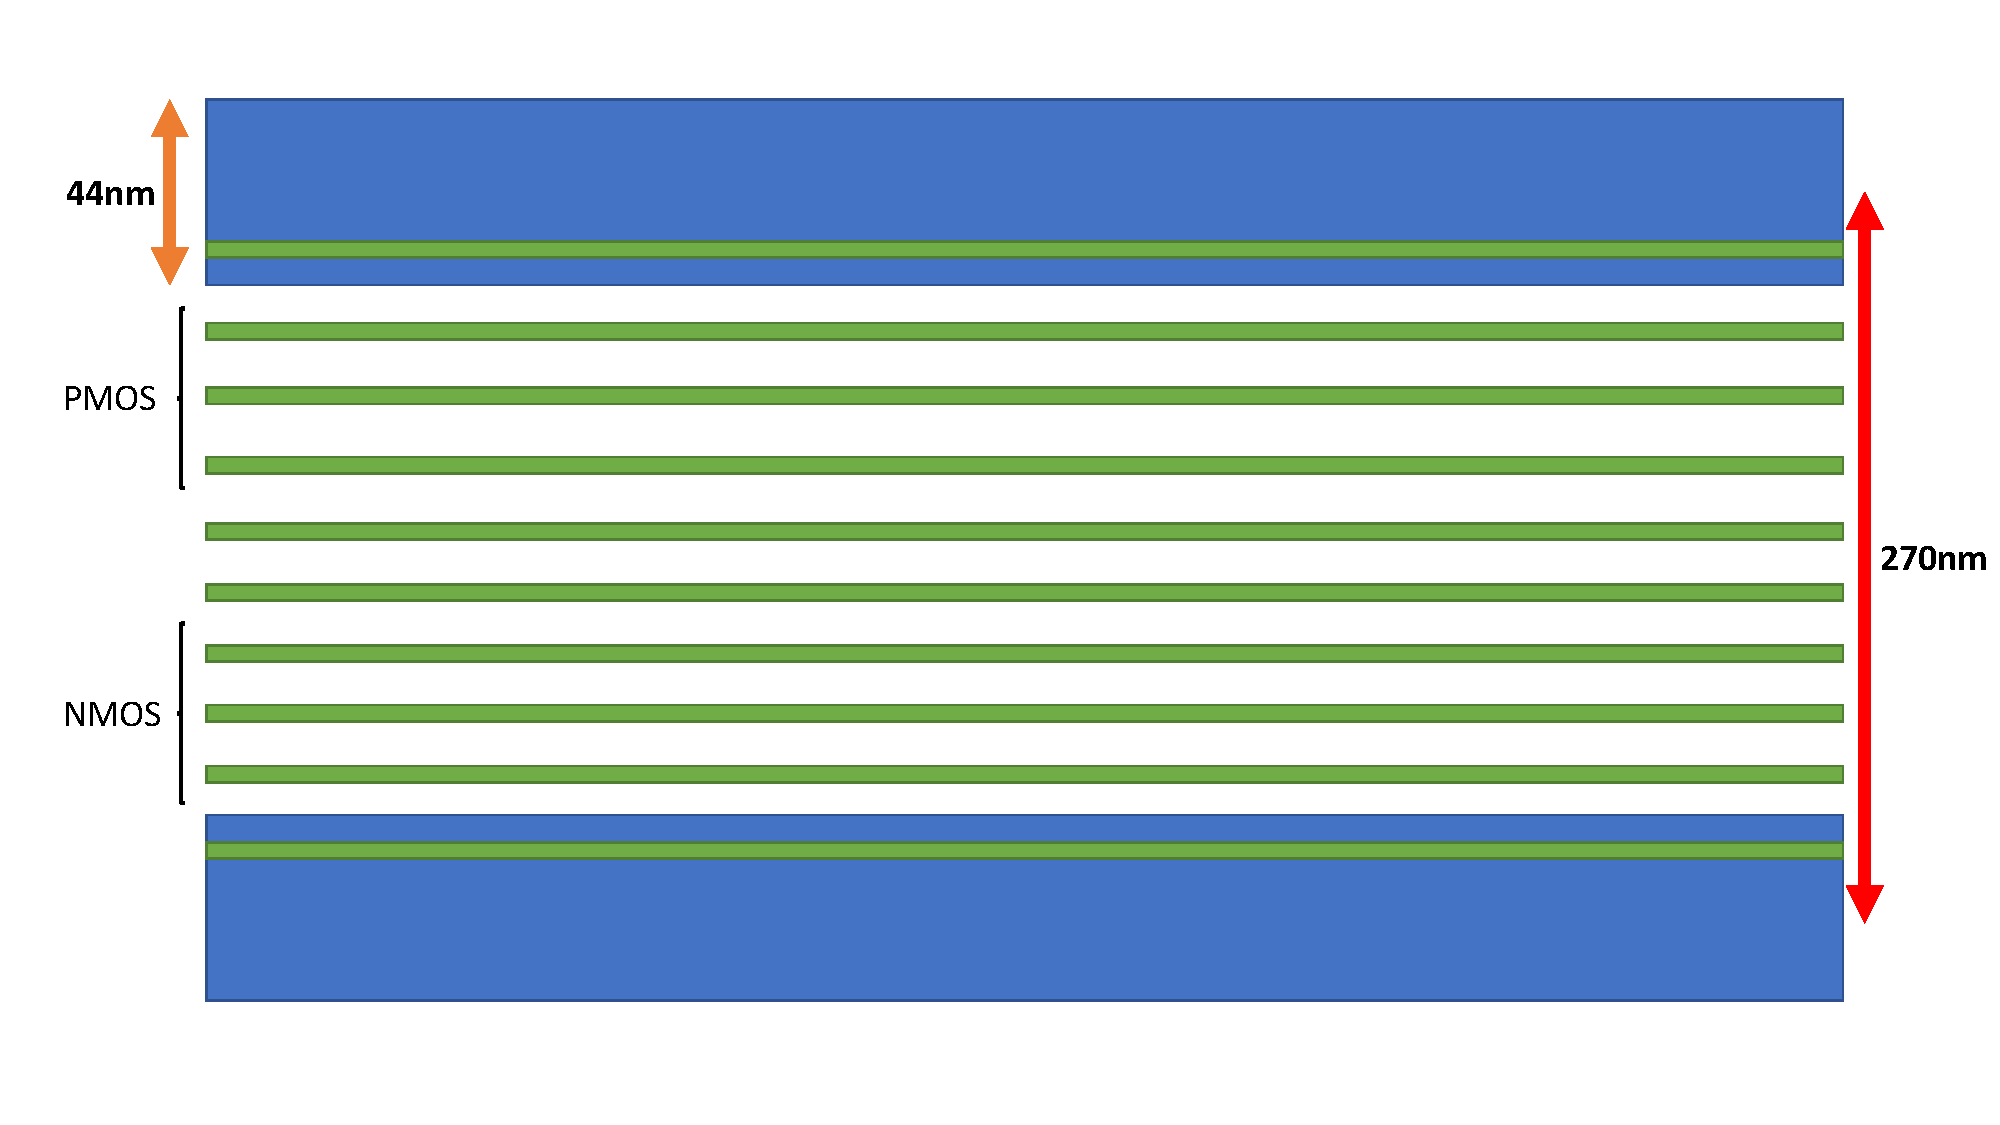
\includegraphics[width=0.8\textwidth]{transistorHeight.pdf}
\caption{Transistor height and number of fins.}
\label{th}
\legend{Source: from author.}
\end{figure}

\begin{figure}[H]
\centering
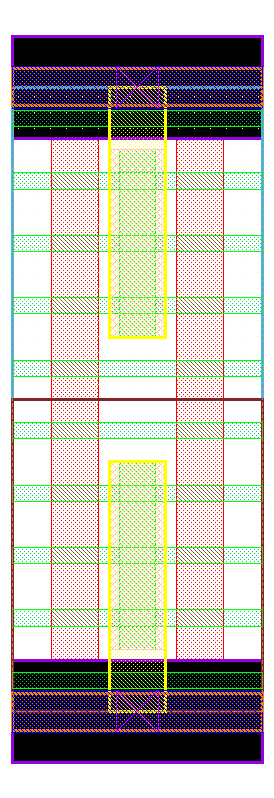
\includegraphics[width=0.2\textwidth]{TAP.png}
\caption{TAP-Cell Layout.}
\label{tap}
\legend{Source: from author.}
\end{figure}

\section{Electrical Simulation}

The simulations were carried out in HSPICE considering the new netlist obtained after the physical verification flow and the parasitic capacitances extraction. Each full adder was designed with and without the Schmitt Triggers replacement to consider the penalties due to the adoption of the ST technique in terms of area, energy and performance. There was performed simulations at nominal supply level (0.7V) and near-threshold level (0.4V) with a frequency of 1GHz for the signals. 

The process variability evaluation was taken, after the layout parasitic extraction through Calibre\textregistered{} from Mentor Graphics, through 2000 Monte Carlo (MC) simulations \cite{2000Simulations} varying the threshold voltage of the PMOS and NMOS devices according to a Gaussian distribution considering a 3\(\sigma\) deviation of 5\% variation from the WFF nominal values. For all experiments, it was observed maximum values, mean (\(\mu\)), standard deviation (\(\sigma\)) and normalized standard deviation (\(\sigma\)/\(\mu\)) for each metric: delay, power and energy, where \(\sigma\)/\(\mu\) represents the sensibility of the cell to process variability. 

The reference values from ASAP7 technology for electrical simulations are shown in Table \ref{electPar}. To avoid underestimating effects of realistic input waveforms on design metrics, the simulations were carried under a 5-bit ripple carry adder using copies of the 1-bit full adder cell with design metrics being calculated for the middle cell as shown in Figure \ref{fig:Fig6}. 

\begin{table}[H]
\centering
\caption{Parameters applied in the electrical simulations}
\label{electPar}
\begin{tabular}{lcc}
\hline
\textbf{Parameter}                                            & \multicolumn{2}{c}{\textbf{7nm}}                                  \\ \hline
\textbf{Nominal Supply Voltage}                               & \multicolumn{2}{c}{0.7 V}                                         \\ \hline
\textbf{Gate Length (L\textsc{g})}           & \multicolumn{2}{c}{21nm}                                          \\ \hline
\textbf{Fin Width (W\textsc{fin})}              & \multicolumn{2}{c}{6.5nm}                                         \\ \hline
\textbf{Fin Height (H\textsc{fin})}          & \multicolumn{2}{c}{32nm}                                          \\ \hline
\textbf{Oxide Thickness (T\textsc{ox})}      & \multicolumn{2}{c}{2.1nm}                                         \\ \hline
\textbf{Channel Doping}                                       & \multicolumn{2}{c}{1x10^{22}m^{-3}}                                     \\ \hline
\textbf{Source/Drain Doping}                                  & \multicolumn{2}{c}{2x10^{22}m^{-3}} \\ \hline
\multicolumn{1}{c}{\multirow{2}{*}{\textbf{Work Function}}} & NFET                            & 4.372                            \\ \cline{2-3} 
\multicolumn{1}{c}{}                                        & PFET                            & 4.8108                           \\ \hline
\end{tabular}
\legend{Source: \citet{clark2016asap7}}
\end{table}

\begin{figure}[H]
\centering
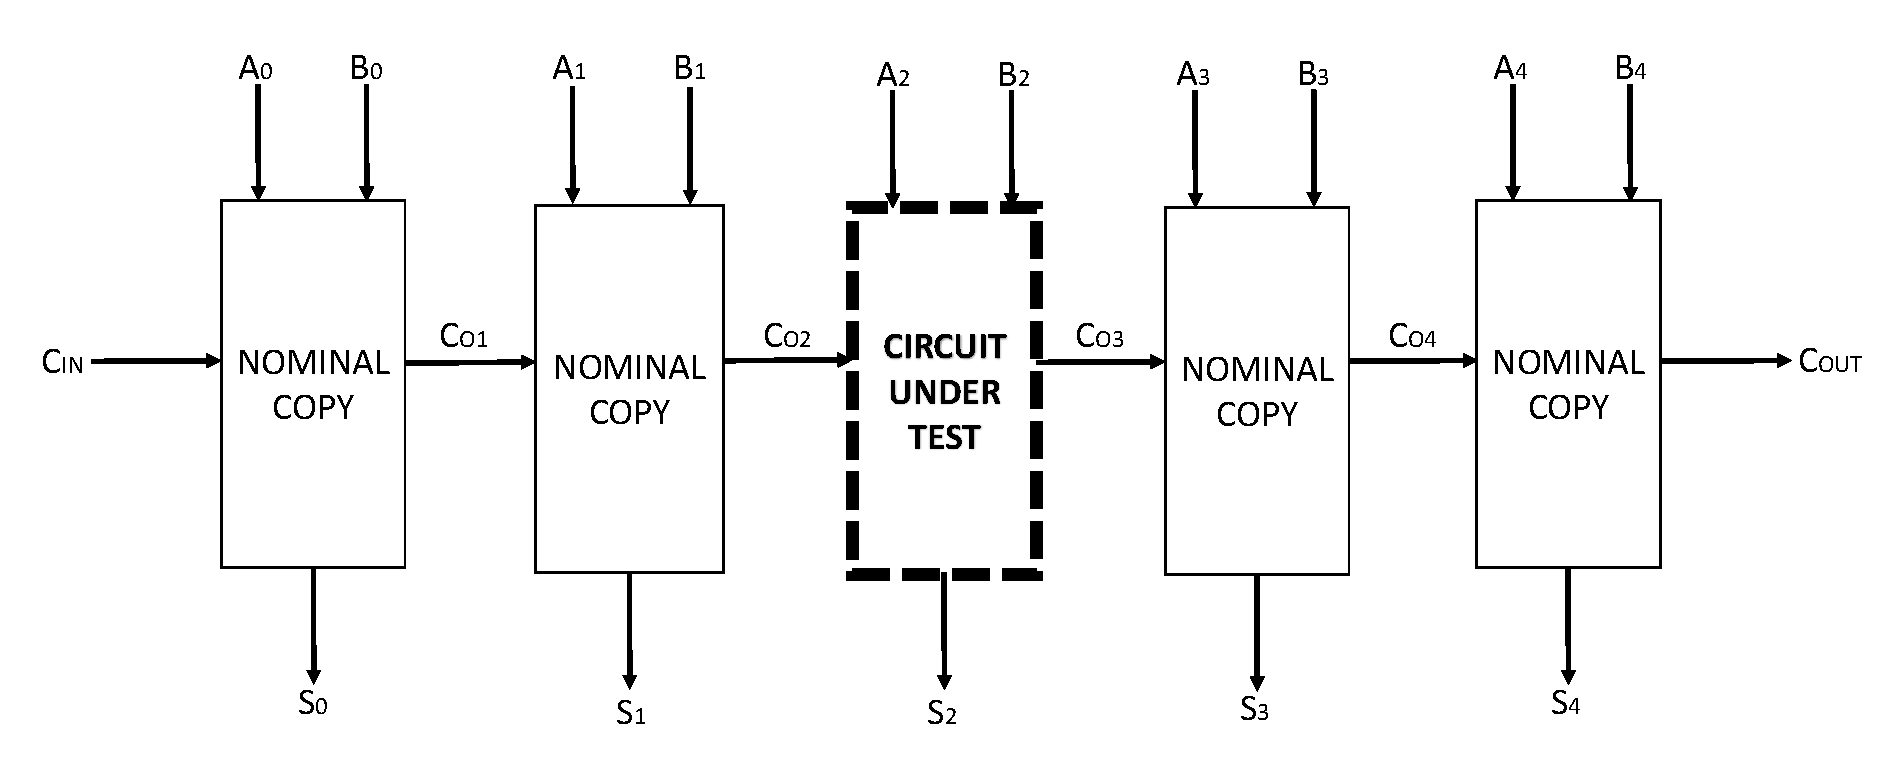
\includegraphics[width=\textwidth]{testbench.pdf}
\caption{Test Bench.}
\label{fig:Fig6}
\legend{Source: \citet{dokania2015circuit}}
\end{figure}



\chapter{Results and Discussion}

The results are organized into two main analysis: the set of full adders were evaluated at nominal voltage conditions and operating at a near-threshold (Nt) region with supply voltage equal to 0.4V. In both cases, the process variability is considered and simulations with and without the ST technique is performed. To highlight the improvements and drawbacks of the ST technique for each FA, results also show the relation (\(\Delta\)) between the deviation of traditional and ST circuits. For each output (Sum and Carry Out) delays and energy measures were considered. All analysis was made at layout level with the 7nm ASAP technology node, with all parasitics considered. 

% \begin{figure}[H]
% \centering
% 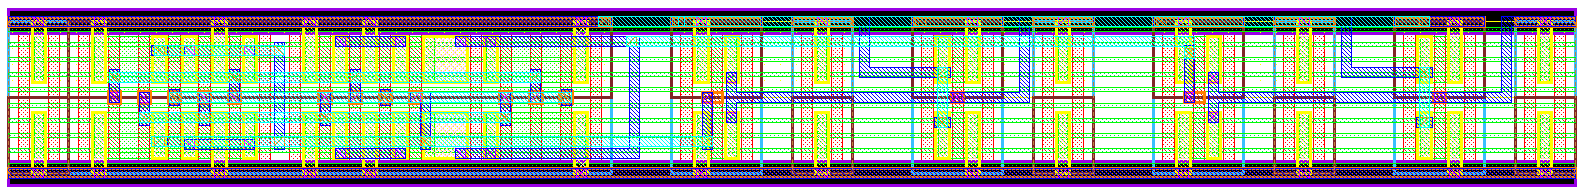
\includegraphics[width=\textwidth]{CMOSST.png}
% \caption{Mirror CMOS Layout with the applied technique.}
% \label{fig:CMOSST}
% \legend{Source: from Author}
% \end{figure}

% \begin{figure}[H]
% \centering
% 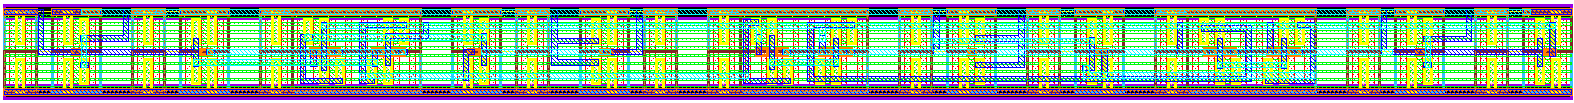
\includegraphics[width=\textwidth]{TGAST.png}
% \caption{TGA Layout with the applied technique.}
% \label{fig:TGAST}
% \legend{Source: from Author}
% \end{figure}

% \begin{figure}[H]
% \centering
% 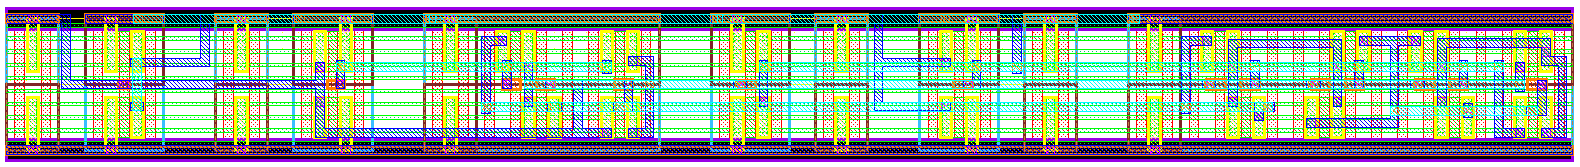
\includegraphics[width=\textwidth]{TFAST.png}
% \caption{TFA Layout with the applied technique.}
% \label{fig:TFAST}
% \legend{Source: from Author}
% \end{figure}

% \begin{figure}[H]
% \centering
% 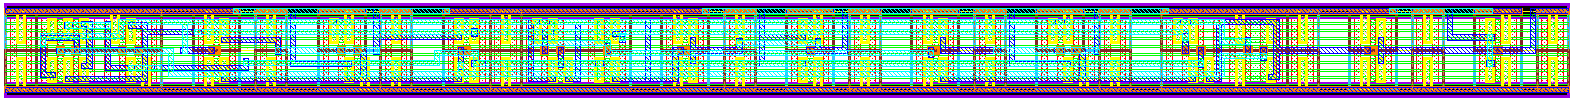
\includegraphics[width=\textwidth]{HYBRIDST.png}
% \caption{Hybrid FA Layout with the applied technique.}
% \label{fig:HYBRIDST}
% \legend{Source: from Author}
% \end{figure}


\section{Nominal Voltage Operation}

At nominal supply voltage, carry-out generation is always the critical path, considering or not the variability effects. According to the Table \ref{delaysNominal} and Table \ref{energyNominal}, it is possible to observe an increase on the mean of delay and energy for all circuits when the ST technique is inserted in the design compared to traditional one.

TFA presented the best performance and the lowest energy consumption for nominal voltage operation. However, TFA presented high maximum values and large standard deviation that are essential points to be considered. These points are a consequence of the heavy signal degradation on the TFA outputs, leaving the TFA for high-performance applications more indicated to technology nodes with low process variability sensibility. The CMOS adder showed the smallest standard deviations being the most recommended for technology nodes with high variability. 

The TGA showed the lowest maximum delays, resulting from the lowest average absolute standard deviations. Although, not presenting the lowest normalized deviation. The Hybrid showed high values for maximum delays (only after the TFA maximum) and the highest mean delays.   

For delays, there was improvement over the Sum (Carry Out) output for the TFA (TGA) with a 37.43\% (15.77\%) higher variability robustness. The CMOS and Hybrid FAs did not show any considerable improvement/worsening. Although, the Carry Out (Sum) output for the TFA (TGA) showed a 25.64\% (11.65\%) robustness worsening.

The results obtained in this work are in the face of the results found to 16nm Predictive Technology Model (PTM) High-Performance technology \cite{ptm} in \cite{samuel2016}. 7nm layout with ASAP7 technology shows significant improvement on the energy robustness (over 18\%) at nominal voltage and in some cases also in the delay robustness to process variability. 

According to Table \ref{energyNominal}, ST circuits increased the mean energy about close two times considering the energy necessary to cover all timing arches to the SUM output. The effect is lighter on the Carry-Out total energy. But, although this penalty, the benefits of ST technique on the cell robustness against process variability are considerable. All the ST FA circuits have the deviation reduced. Hybrid presented the best improvement on energy robustness, with 30\% more stability. Fig. \ref{fig:improvNominal} resumes the improvement reached with the ST technique on Delay and Energy.

\begin{table}[!htbp]
\centering
\caption{Delay measures for nominal voltage operation.}
\label{delaysNominal}
\resizebox{\textwidth}{!}{%
\begin{tabular}{lcccccccccc}
\hline
\multirow{3}{*}{@Nominal Voltage} & \multicolumn{10}{c}{Delay}                                                                                                                                                                                     \\ \cline{2-11} 
                                  & \multicolumn{5}{c}{SUM}                                                                               & \multicolumn{5}{c}{CARRY OUT}                                                                         \\ \cline{2-11} 
                                  & Max (ps)              &  \(\mu\) (ps)          & \(\sigma\) (ps)          & \(\sigma\)/\(\mu\) (\%)      & \(\Delta\) (\%)                           & Max (ps)               & \(\mu\) (ps)           & \(\sigma\) (ps)          & \(\sigma\)/\(\mu\) (\%)      & \(\Delta\) (\%)                           \\ \hline
\textbf{CMOS}                     & 93.19            & 16.11          & 3.83           & 23.31          & \multirow{2}{*}{4.46}            & 104.48           & 27.38          & 5.92           & 21.60          & \multirow{2}{*}{1.05}            \\ \cline{1-5} \cline{7-10}
\textbf{CMOS ST}                  & 117.19           & 21.98          & 4.98           & \textbf{22.27} &                                  & 120.01           & \textbf{33.09} & 7.08           & \textbf{21.38} &                                  \\ \hline
\textbf{TGA}                      & \textbf{63.13}   & 14.51          & \textbf{3.28}  & 27.94          & \multirow{2}{*}{\textbf{-11.65}} & \textbf{60.11}   & 16.32          & 4.28           & 28.54          & \multirow{2}{*}{\textbf{15.77}}  \\ \cline{1-5} \cline{7-10}
\textbf{TGA ST}                   & 77.71            & 17.63          & 3.80           & 31.20          &                                  & 71.82            & 21.19          & 4.77           & 24.04          &                                  \\ \hline
\textbf{TFA}                      & \textbf{1016.90} & \textbf{12.63} & \textbf{10.62} & \textbf{58.94} & \multirow{2}{*}{\textbf{37.43}}  & 2010.20          & \textbf{14.74} & 13.77          & 77.59          & \multirow{2}{*}{\textbf{-25.64}} \\ \cline{1-5} \cline{7-10}
\textbf{TFA ST}                   & 83.52            & 15.39          & 4.16           & 36.88          &                                  & \textbf{2030.50} & 22.72          & \textbf{37.42} & \textbf{97.48} &                                  \\ \hline
\textbf{HYBRID}                   & 117.57           & 18.15          & 4.42           & 23.72          & \multirow{2}{*}{-0.75}           & 65.29            & 17.30          & \textbf{4.18}  & 25.57          & \multirow{2}{*}{4.20}            \\ \cline{1-5} \cline{7-10}
\textbf{HYBRID ST}                & 192.48           & \textbf{25.92} & 6.55           & 23.90          &                                  & 96.40            & 23.27          & 5.64           & 24.50          &                                  \\ \hline
\end{tabular}%
}
\end{table}


% Please add the following required packages to your document preamble:
% \usepackage{multirow}
% \usepackage{graphicx}
\begin{table}[!htbp]
\centering
\caption{Energy measures for nominal voltage operation.}
\label{energyNominal}
\resizebox{\textwidth}{!}{%
\begin{tabular}{lcccccccccc}
\hline
\multirow{3}{*}{@Nominal Voltage} & \multicolumn{10}{c}{Energy}                                                                                                                                                                            \\ \cline{2-11} 
                                  & \multicolumn{5}{c}{SUM}                                                                           & \multicolumn{5}{c}{CARRY OUT}                                                                     \\ \cline{2-11} 
                                  & Max (fJ)              &  \(\mu\) (fJ)          & \(\sigma\) (fJ)          & \(\sigma\)/\(\mu\) (\%)      & \(\Delta\) (\%)                           & Max (fJ)               & \(\mu\) (fJ)           & \(\sigma\) (fJ)          & \(\sigma\)/\(\mu\) (\%)      & \(\Delta\) (\%)                          \\ \hline
\textbf{CMOS}                     & 69.07          & 12.89          & 2.97          & 23.00          & \multirow{2}{*}{18.21}          & 83.43          & 20.88          & 3.52          & 16.87          & \multirow{2}{*}{\textbf{18.91}} \\ \cline{1-5} \cline{7-10}
\textbf{CMOS ST}                  & \textbf{93.07} & 20.26          & 3.81          & 18.81          &                                 & 98.66          & 30.69          & 4.20          & 13.68          &                                 \\ \hline
\textbf{TGA}                      & 60.36          & 11.78          & 2.36          & 20.04          & \multirow{2}{*}{\textbf{3.71}}  & 92.71          & 13.54          & 4.15          & \textbf{30.61} & \multirow{2}{*}{\textbf{31.32}} \\ \cline{1-5} \cline{7-10}
\textbf{TGA ST}                   & 90.61          & 22.99          & \textbf{4.44} & 19.30          &                                 & 93.03          & 24.79          & \textbf{5.21} & 21.03          &                                 \\ \hline
\textbf{TFA}                      & \textbf{21.94} & \textbf{4.45}  & \textbf{0.92} & 20.67          & \multirow{2}{*}{33.73}          & \textbf{29.74} & \textbf{4.96}  & \textbf{1.14} & 22.99          & \multirow{2}{*}{19.62}          \\ \cline{1-5} \cline{7-10}
\textbf{TFA ST}                   & 29.28          & 10.59          & 1.45          & \textbf{13.70} &                                 & 53.74          & 10.58          & 1.96          & 18.48          &                                 \\ \hline
\textbf{HYBRID}                   & 86.45          & 12.99          & 3.63          & \textbf{27.97} & \multirow{2}{*}{\textbf{37.38}} & 93.88          & 19.99          & 3.89          & 19.48          & \multirow{2}{*}{29.74}          \\ \cline{1-5} \cline{7-10}
\textbf{HYBRID ST}                & 87.13          & \textbf{23.67} & 4.15          & 17.52          &                                 & \textbf{98.85} & \textbf{35.58} & 4.87          & \textbf{13.69} &                                 \\ \hline
\end{tabular}%
}
\end{table}

\begin{figure}[H]
\centering
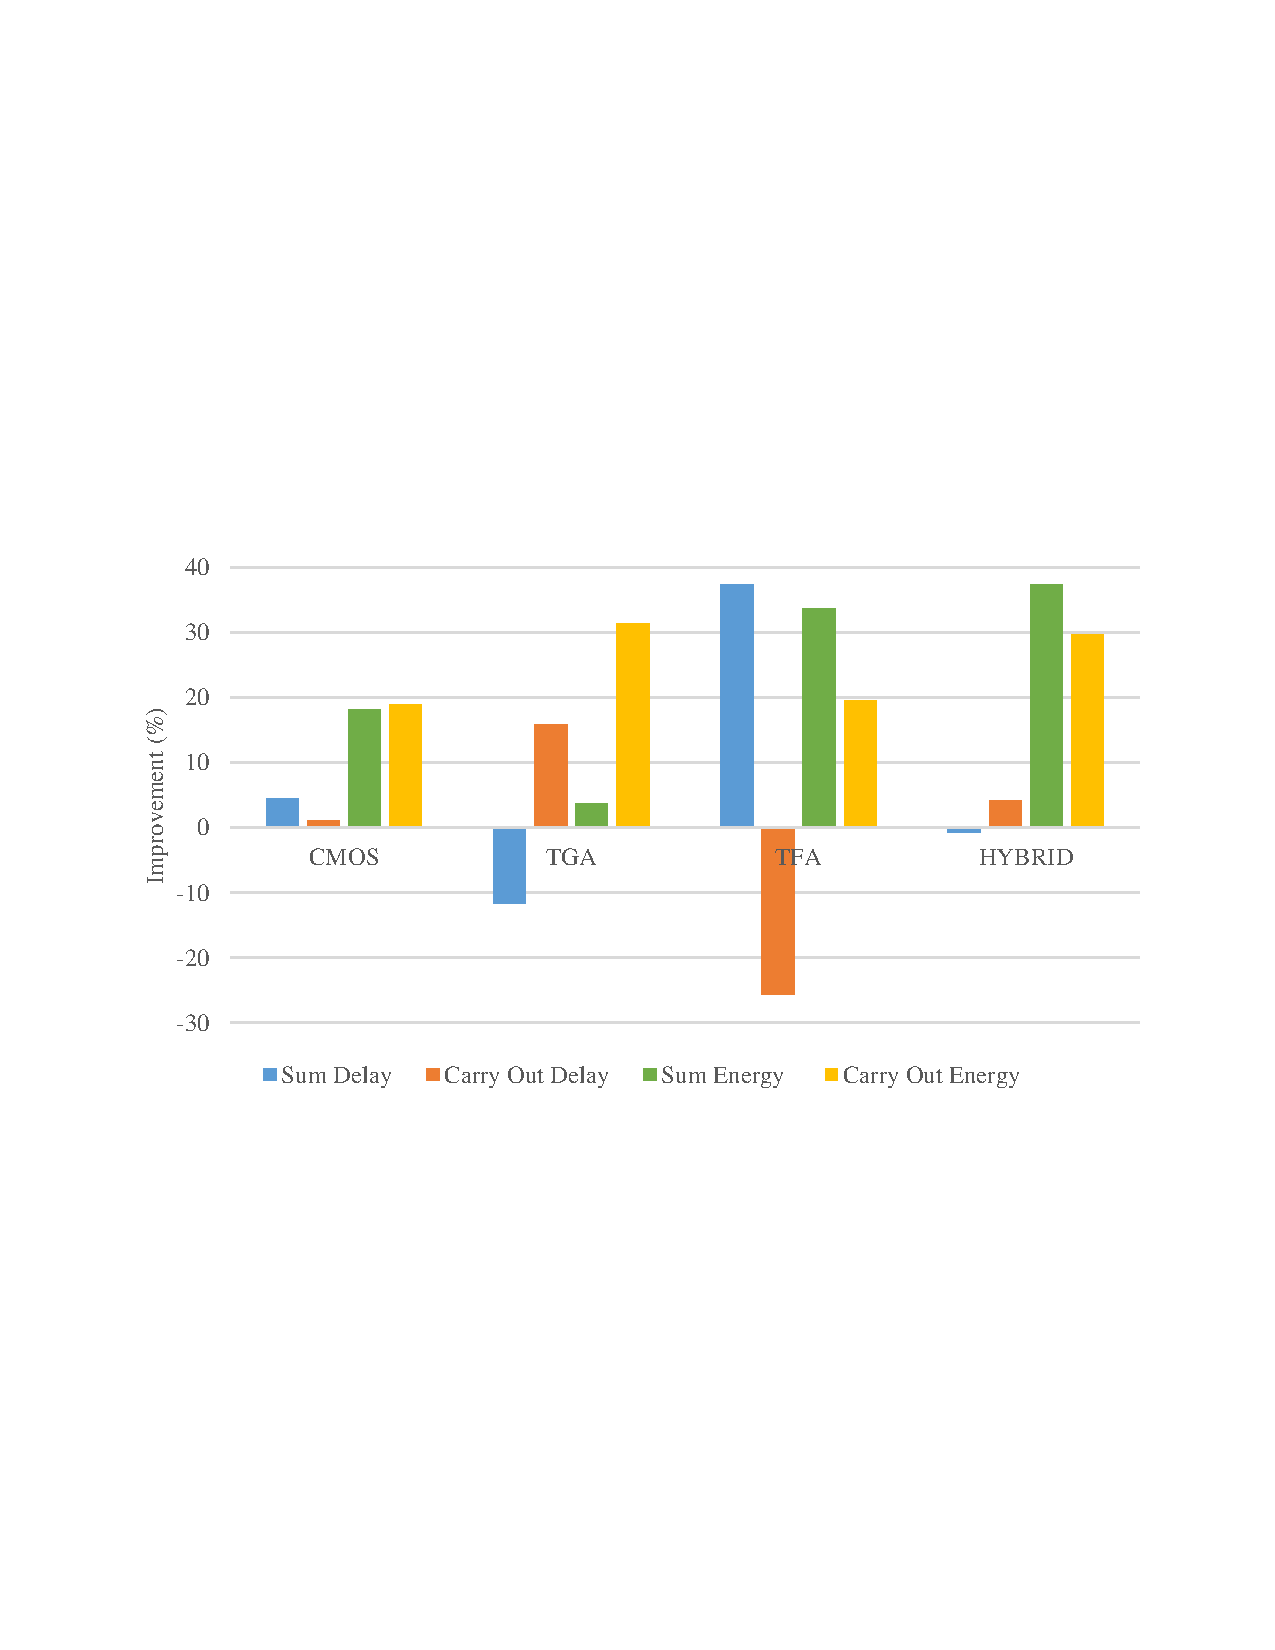
\includegraphics[width=\textwidth, trim={0 9cm 0 9cm},clip]{improvNominal.pdf}
\caption{Robustness improvements for each Full Adder at nominal voltage operation.}
\label{fig:improvNominal}
\legend{Source: from author.}
\end{figure}

\section{Near-Threshold Operation}

At near-threshold, variability compromises the FA circuits on some cases making the SUM output the critical path instead of the Carry-out generation, observing the maximum values found. Table \ref{delaysNT} presents the delay results of the near-threshold operation. 

The energy results to near-threshold operation are presented in Table \ref{energyNT}. Operating at low voltage reduces the mean energy over 30\% for CMOS, TFA and Hybrid FAs and at least 15\% of TGA compared to nominal voltage operation. As stated on \cite{dokania2015circuit}, the ST technique at NT operation reduces the delay and energy deviation for all circuits. However, the lag of the circuits is considerably higher at NT operation, emphasizing the need of circuit strategies to deal with variability. 

TFA and TGA showed the highest deviations and high maximum delays, which is expected due to their pass-transistor logic and inherent signal degradation. The Hybrid adder showed higher deviations, delays and similar energy consumption in comparison to the CMOS Adder. Given that, the CMOS adder remains as a good choice for low power applications.

Results make clear the advantage of the technique when considering energy variability robustness. Fig. \ref{fig:NTimprov} shows the comparative evaluation of the improvement reached by ST technique at NT operation. Even when there was a worsening on delay robustness, the energy robustness presented improvements. The technique can introduce more delay variability given that variability determines the ST behavior as well, influencing its delays, which stacks with the impact of multiple transistors in a series arrangement.

\begin{table}[!htbp]
\centering
\caption{Delay measures for near-threshold operation.}
\label{delaysNT}
\resizebox{\textwidth}{!}{%
\begin{tabular}{lcccccccccc}
\hline
\multicolumn{1}{c}{\multirow{3}{*}{@NT}} & \multicolumn{10}{c}{Delay}                                                                                                                                                                                          \\ \cline{2-11} 
\multicolumn{1}{c}{}                     & \multicolumn{5}{c}{SUM}                                                                                 & \multicolumn{5}{c}{CARRY OUT}                                                                            \\ \cline{2-11} 
\multicolumn{1}{c}{}                     & Max (ps)              &  \(\mu\) (ps)          & \(\sigma\) (ps)          & \(\sigma\)/\(\mu\) (\%)      & \(\Delta\) (\%)                           & Max (ps)               & \(\mu\) (ps)           & \(\sigma\) (ps)          & \(\sigma\)/\(\mu\) (\%)      & \(\Delta\) (\%)                           \\ \hline
\textbf{CMOS}                              & 873.41           & 73.22           & \textbf{56.38}  & 77.47           & \multirow{2}{*}{18.70}          & 794.87           & 128.65          & 86.67           & 67.39           & \multirow{2}{*}{11.61}           \\ \cline{1-5} \cline{7-10}
\textbf{CMOS ST}                           & \textbf{430.85}  & 95.85           & 60.57           & \textbf{62.99}  &                                 & \textbf{539.77}  & 143.77          & 85.67           & 59.57           &                                  \\ \hline
\textbf{TGA}                               & \textbf{7328.30} & \textbf{62.90}  & 92.17           & 133.30          & \multirow{2}{*}{31.53}          & 6396.90          & \textbf{325.25} & 138.02          & 173.54          & \multirow{2}{*}{-19.14}          \\ \cline{1-5} \cline{7-10}
\textbf{TGA ST}                            & 2386.40          & \textbf{127.54} & \textbf{106.22} & 91.26           &                                 & 6265.10          & 181.01          & \textbf{373.37} & 206.76          &                                  \\ \hline
\textbf{TFA}                               & 1024.90          & 67.28           & 93.48           & \textbf{289.41} & \multirow{2}{*}{\textbf{64.74}} & 5734.20          & 151.02          & 286.55          & 227.50          & \multirow{2}{*}{\textbf{-21.16}} \\ \cline{1-5} \cline{7-10}
\textbf{TFA ST}                            & 4202.20          & 84.34           & 79.51           & 102.05          &                                 & \textbf{6705.80} & 94.87           & 233.09          & \textbf{275.63} &                                  \\ \hline
\textbf{HYBRID}                            & 830.64           & 95.23           & 77.95           & 79.00           & \multirow{2}{*}{\textbf{13.43}} & 695.28           & \textbf{78.00}  & \textbf{56.73}  & 73.90           & \multirow{2}{*}{\textbf{19.48}}  \\ \cline{1-5} \cline{7-10}
\textbf{HYBRID ST}                         & 1212.00          & 120.92          & 86.26           & 68.39           &                                 & 2755.30          & 168.92          & 100.34          & \textbf{59.51}  &                                  \\ \hline
\end{tabular}%
}
\end{table}

% Please add the following required packages to your document preamble:
% \usepackage{multirow}
% \usepackage{graphicx}
\begin{table}[!htbp]
\centering
\caption{Energy measures for near-threshold operation.}
\label{energyNT}
\resizebox{\textwidth}{!}{%
\begin{tabular}{lcccccccccc}
\hline
\multicolumn{1}{c}{\multirow{3}{*}{@NT}} & \multicolumn{10}{c}{Energy}                                                                                                                                                                            \\ \cline{2-11} 
\multicolumn{1}{c}{}                     & \multicolumn{5}{c}{SUM}                                                                           & \multicolumn{5}{c}{CARRY OUT}                                                                     \\ \cline{2-11} 
\multicolumn{1}{c}{}                     & Max (fJ)              &  \(\mu\) (fJ)          & \(\sigma\) (fJ)          & \(\sigma\)/\(\mu\) (\%)      & \(\Delta\) (\%)                           & Max (fJ)               & \(\mu\) (fJ)           & \(\sigma\) (fJ)          & \(\sigma\)/\(\mu\) (\%)      & \(\Delta\) (\%)                          \\ \hline
\textbf{CMOS}                              & 45.37          & 6.29           & 2.00          & 31.81          & \multirow{2}{*}{\textbf{20.07}} & 51.91          & 9.97           & 2.09          & 20.97          & \multirow{2}{*}{\textbf{12.02}} \\ \cline{1-5} \cline{7-10}
\textbf{CMOS ST}                           & 60.64          & 10.22          & 2.60          & 25.43          &                                 & 70.97          & \textbf{15.16} & \textbf{2.80} & 18.45          &                                 \\ \hline
\textbf{TGA}                               & 53.90          & 6.06           & 2.01          & 33.17          & \multirow{2}{*}{61.45}          & 61.28          & 6.40           & 1.85          & \textbf{28.90} & \multirow{2}{*}{34.04}          \\ \cline{1-5} \cline{7-10}
\textbf{TGA ST}                            & 34.33          & 11.30          & 1.44          & 12.79          &                                 & \textbf{85.49} & 11.67          & 2.22          & 19.06          &                                 \\ \hline
\textbf{TFA}                               & \textbf{16.26} & \textbf{2.40}  & 0.65          & 27.05          & \multirow{2}{*}{\textbf{66.59}} & 23.03          & \textbf{2.58}  & \textbf{0.64} & 24.66          & \multirow{2}{*}{52.18}          \\ \cline{1-5} \cline{7-10}
\textbf{TFA ST}                            & 18.85          & 5.45           & \textbf{0.49} & \textbf{9.04}  &                                 & \textbf{22.21} & 5.61           & 0.66          & 11.79          &                                 \\ \hline
\textbf{HYBRID}                            & 56.96          & 6.02           & 2.29          & \textbf{38.04} & \multirow{2}{*}{27.06}          & 59.99          & 9.46           & 2.00          & 21.19          & \multirow{2}{*}{\textbf{61.91}} \\ \cline{1-5} \cline{7-10}
\textbf{HYBRID ST}                         & \textbf{81.05} & \textbf{11.65} & \textbf{3.23} & 27.75          &                                 & 26.22          & 15.03          & 1.21          & \textbf{8.07}  &                                 \\ \hline
\end{tabular}%
}
\end{table}

\begin{figure}[!htb]
\centering
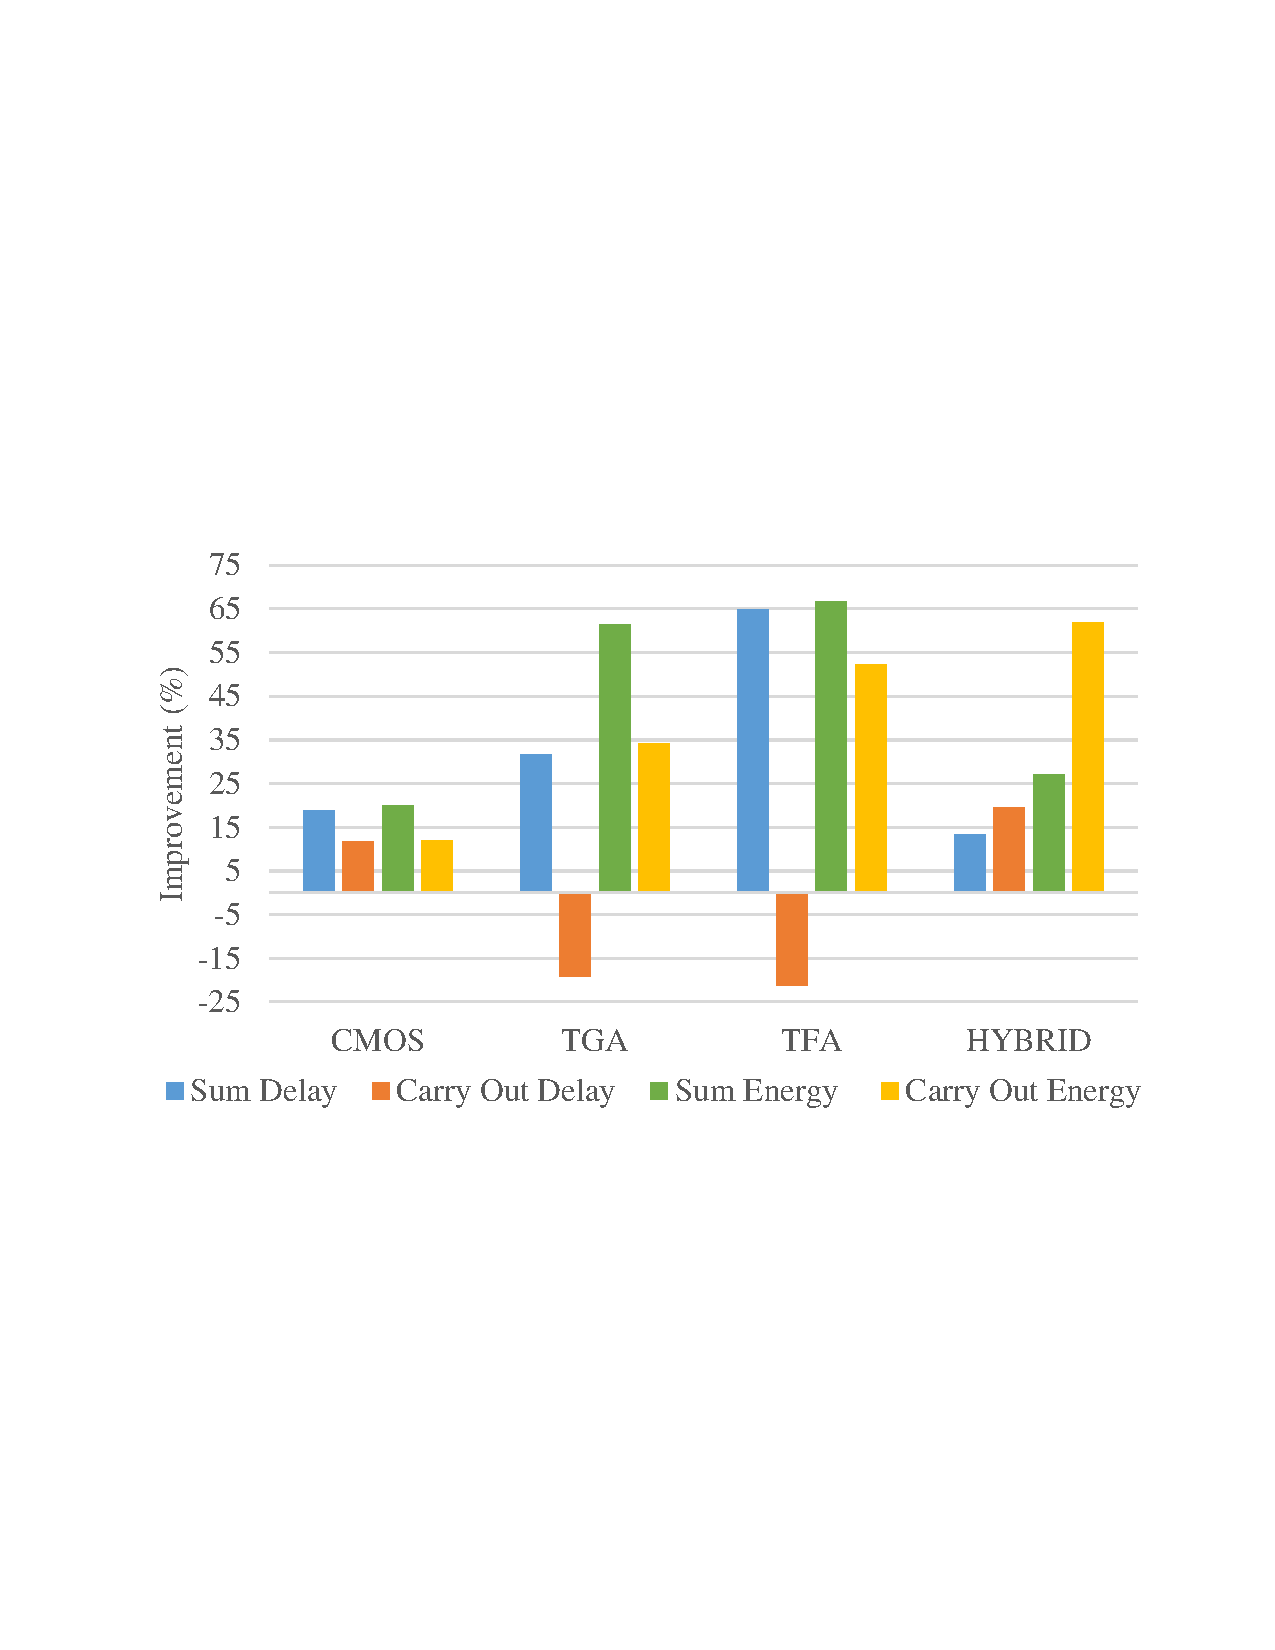
\includegraphics[width=\textwidth, trim={0 9cm 0 9cm},clip]{improvNT.pdf}
\caption{Robustness improvements for each Full Adder at near-threshold operation.}
\label{fig:NTimprov}
\legend{Source: from author.}
%\legend{Source: \cite{dokania2015circuit}}
\end{figure}

\section{Penalties}

It is expected that a technique which replaces a 2-transistor sub-circuit to a 4-transistor one should bring an impact over metrics. Given so, the average impact at nominal voltage operation was 30\% over the delay and their absolute deviation values for nominal voltage and near-threshold operations. For nominal voltage operation, both outputs had similar penalties (35\% increase in delays). For near-threshold operation the Sum output had a considerable higher penalty (47\%) in comparison to the Carry Out output (12\%). For delay deviation both operation regimes had similar results with an 8\% increase for the Sum output and a 60\% increase for the Carry Out output, which is expected since Carry Out is the critical path.


For energy, the impact is considerable, being on average over 85\% percent higher. For energy standard deviations there was a 40\% increase at nominal voltage and a minor 4\% increase at near-threshold level. At both operation regimes and at both outputs the penalty for energy was similar, with a 93\% increase for the Sum output and 80\% increase for the Carry Out output. For the energy devation, at nominal voltage operation there was a higher penalty for the Sum output (47\%) in comparison to the Carry Out output (35\%). At near-threshold operation both outputs had the same minor penalty of 4\% on deviations. 

Overall, the worst penalties were the 47\% increase in delays in Sum output at near-threshold operation, 59\% increase on delay deviation in the Carry Out output at nominal operation, 93\% increase at energy consumption for Sum output at both operation regimes and its 47\% increase in energy deviation at nominal operation. Energy penalties are plotted at Figures \ref{fig:energyNS} to \ref{fig:energyNTCO}. 

\begin{figure}[H]
\centering
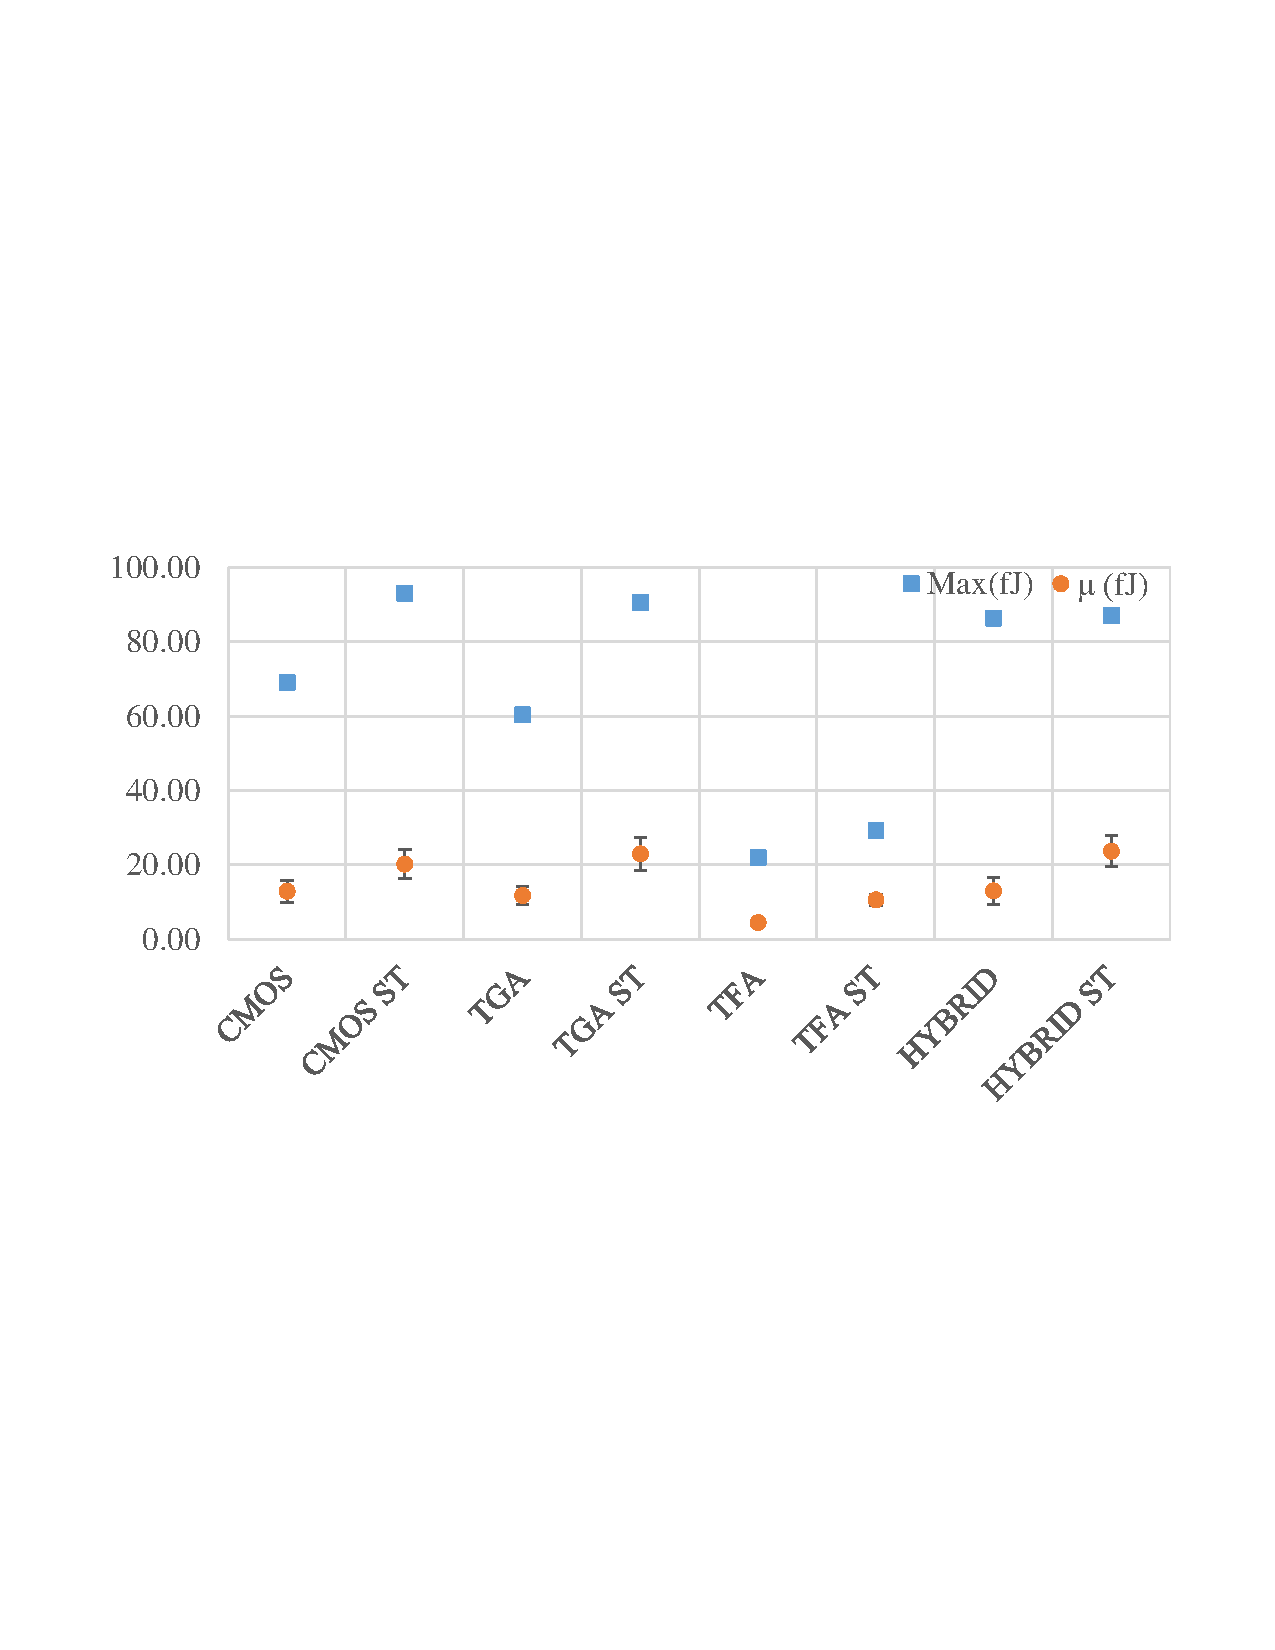
\includegraphics[width=\textwidth, trim={0 9cm 0 9cm},clip]{energyNominalSum.pdf}
\caption{Energy penalties for the Sum output at Nominal voltage operation.}
\label{fig:energyNS}
\legend{Source: from author.}
\end{figure}

\begin{figure}[H]
\centering
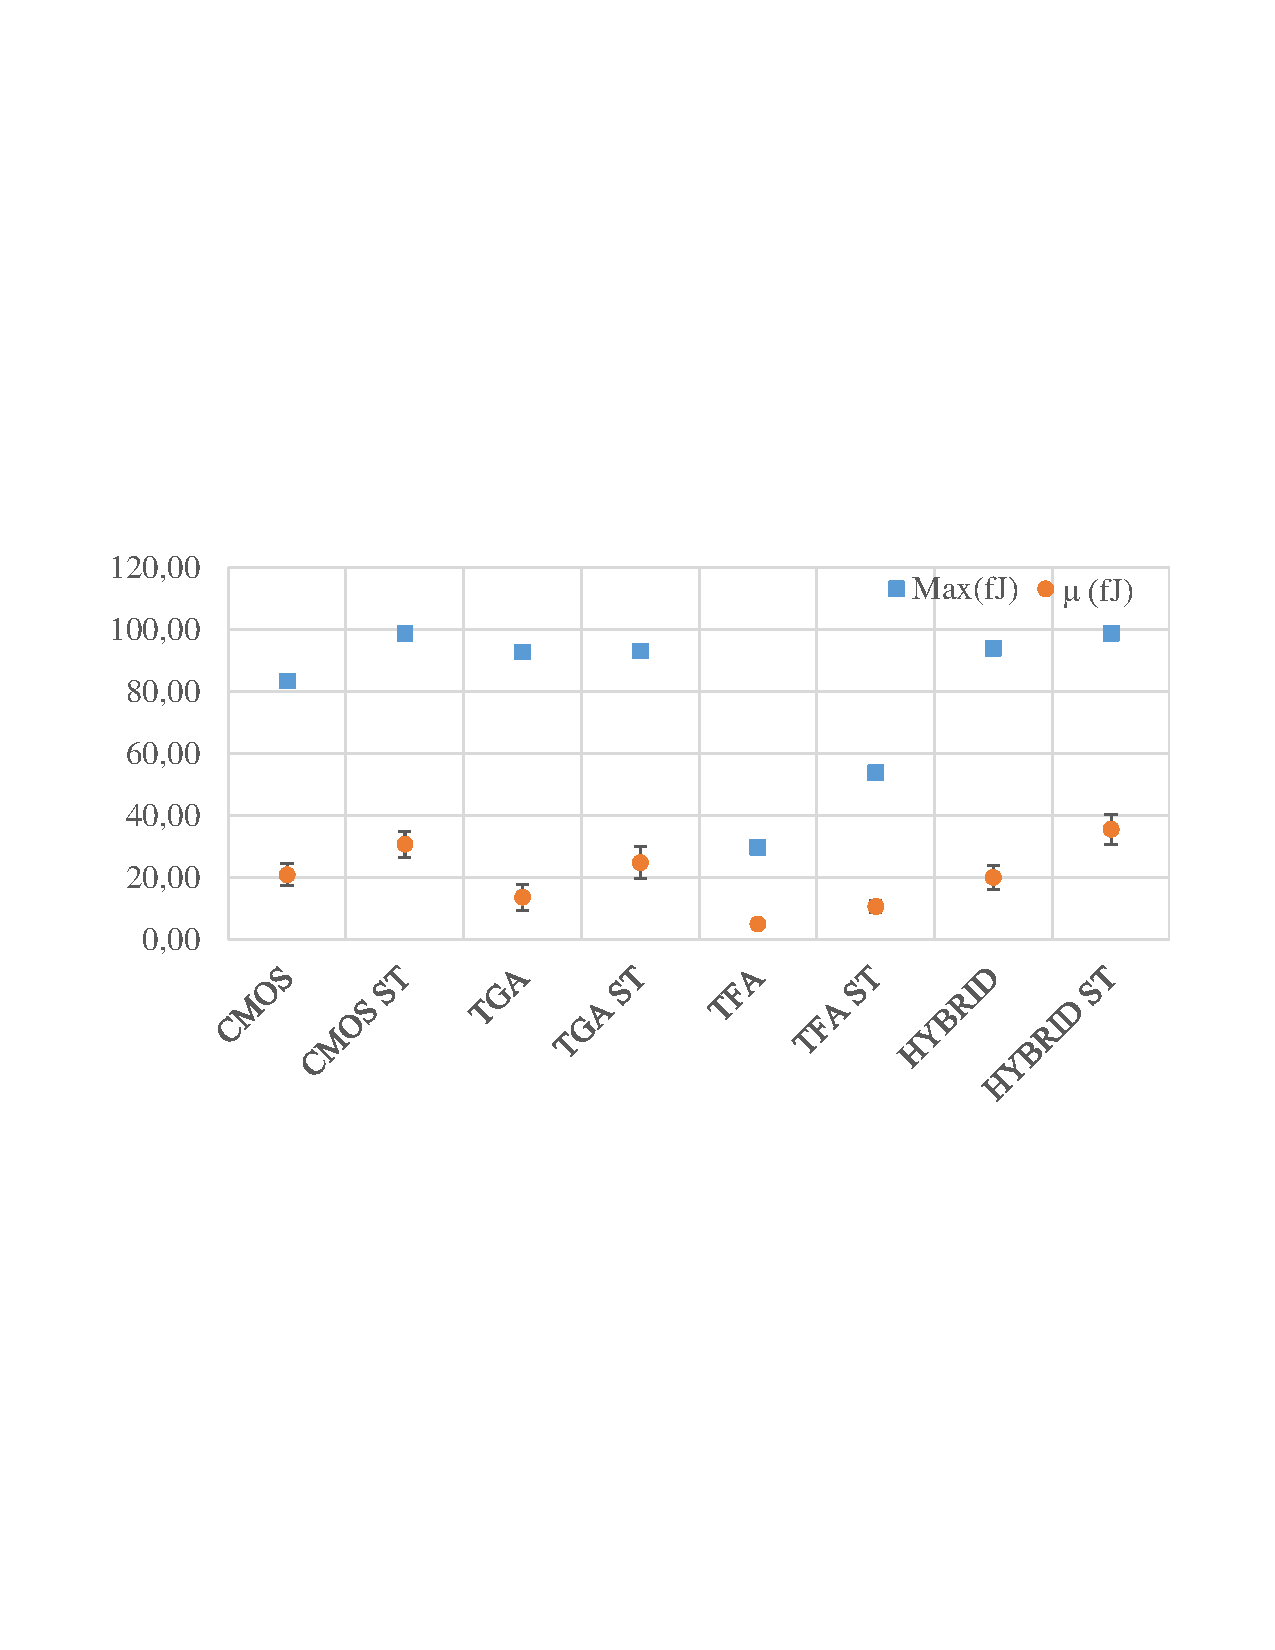
\includegraphics[width=\textwidth, trim={0 9cm 0 9cm},clip]{energyNominalCarryOut.pdf}
\caption{Energy penalties for the Carry Out output at Nominal voltage operation.}
\label{fig:energyNCO}
\legend{Source: from author.}
\end{figure}

\begin{figure}[H]
\centering
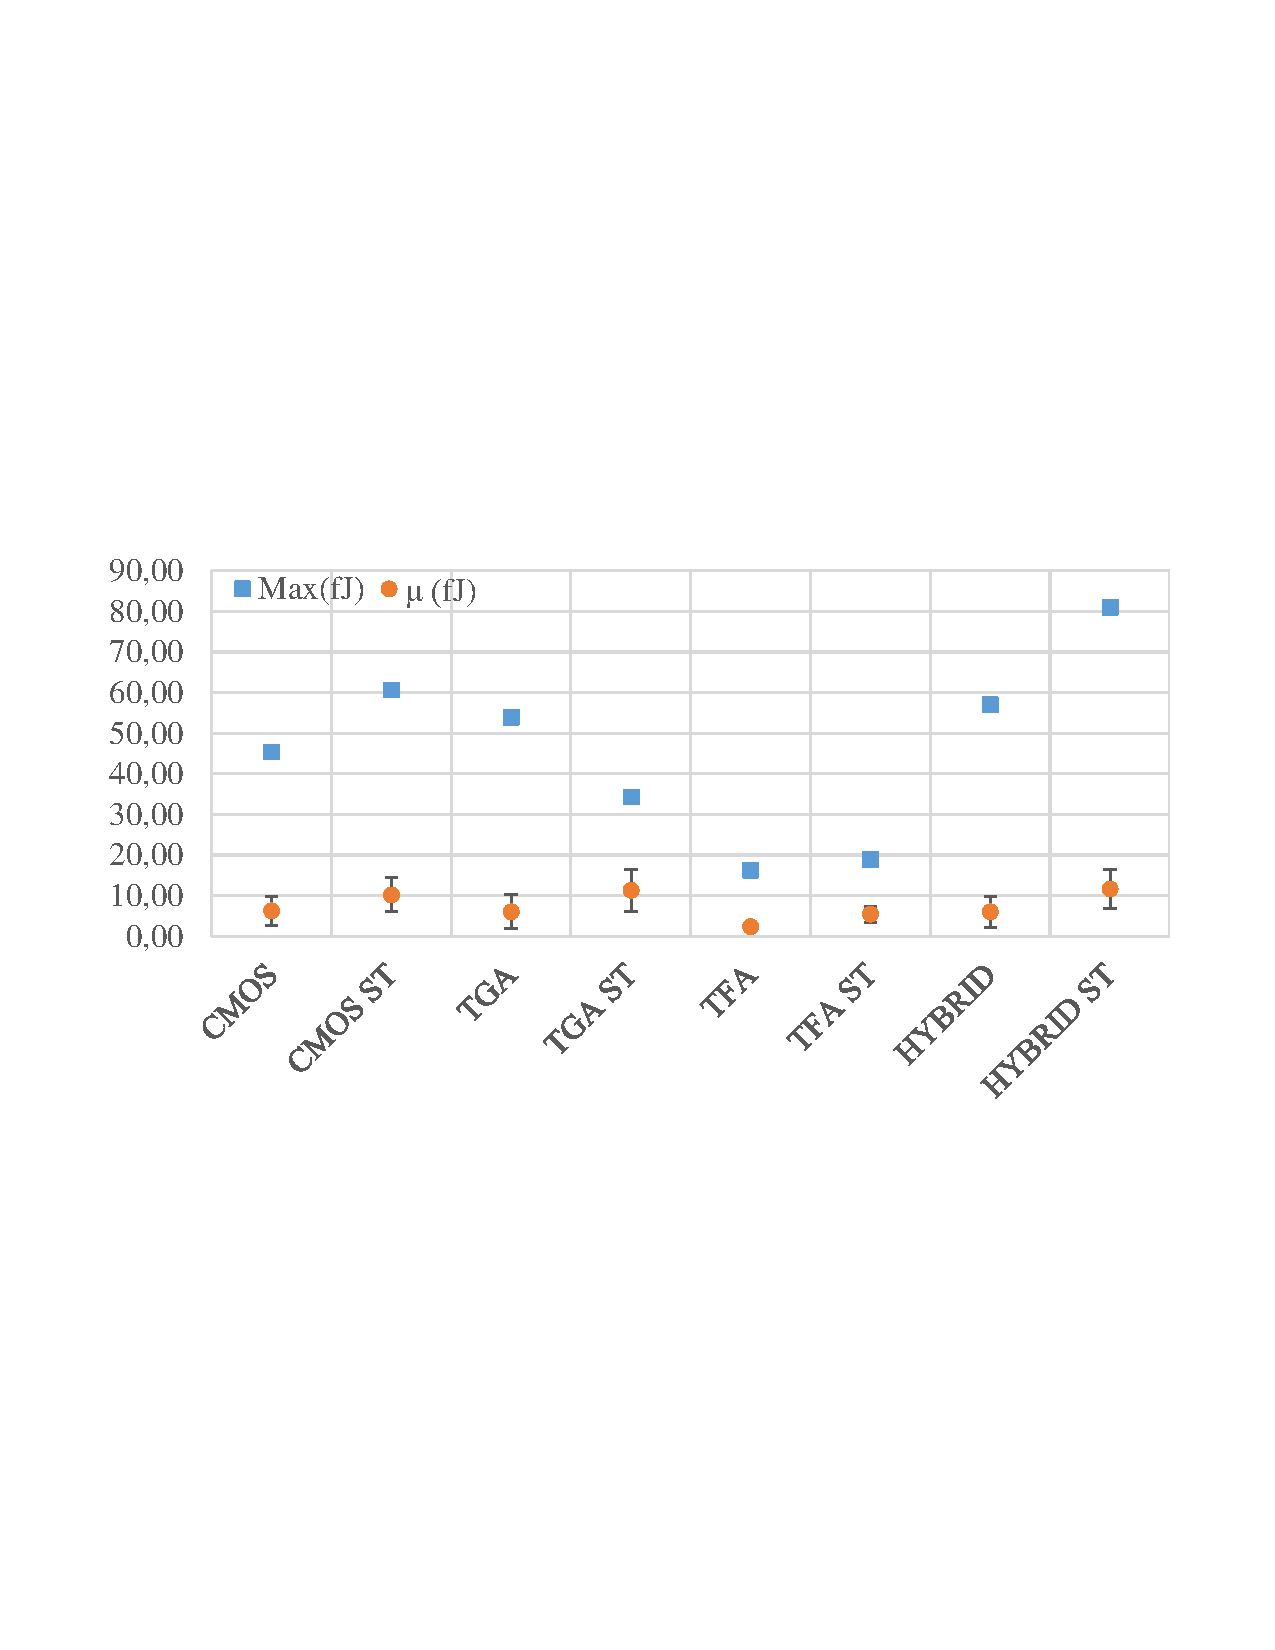
\includegraphics[width=\textwidth, trim={0 9cm 0 9cm},clip]{energyNTSum.pdf}
\caption{Energy penalties for the Sum output at Near-Threshold operation.}
\label{fig:energyNTS}
\legend{Source: from author.}
\end{figure}

\begin{figure}[H]
\centering
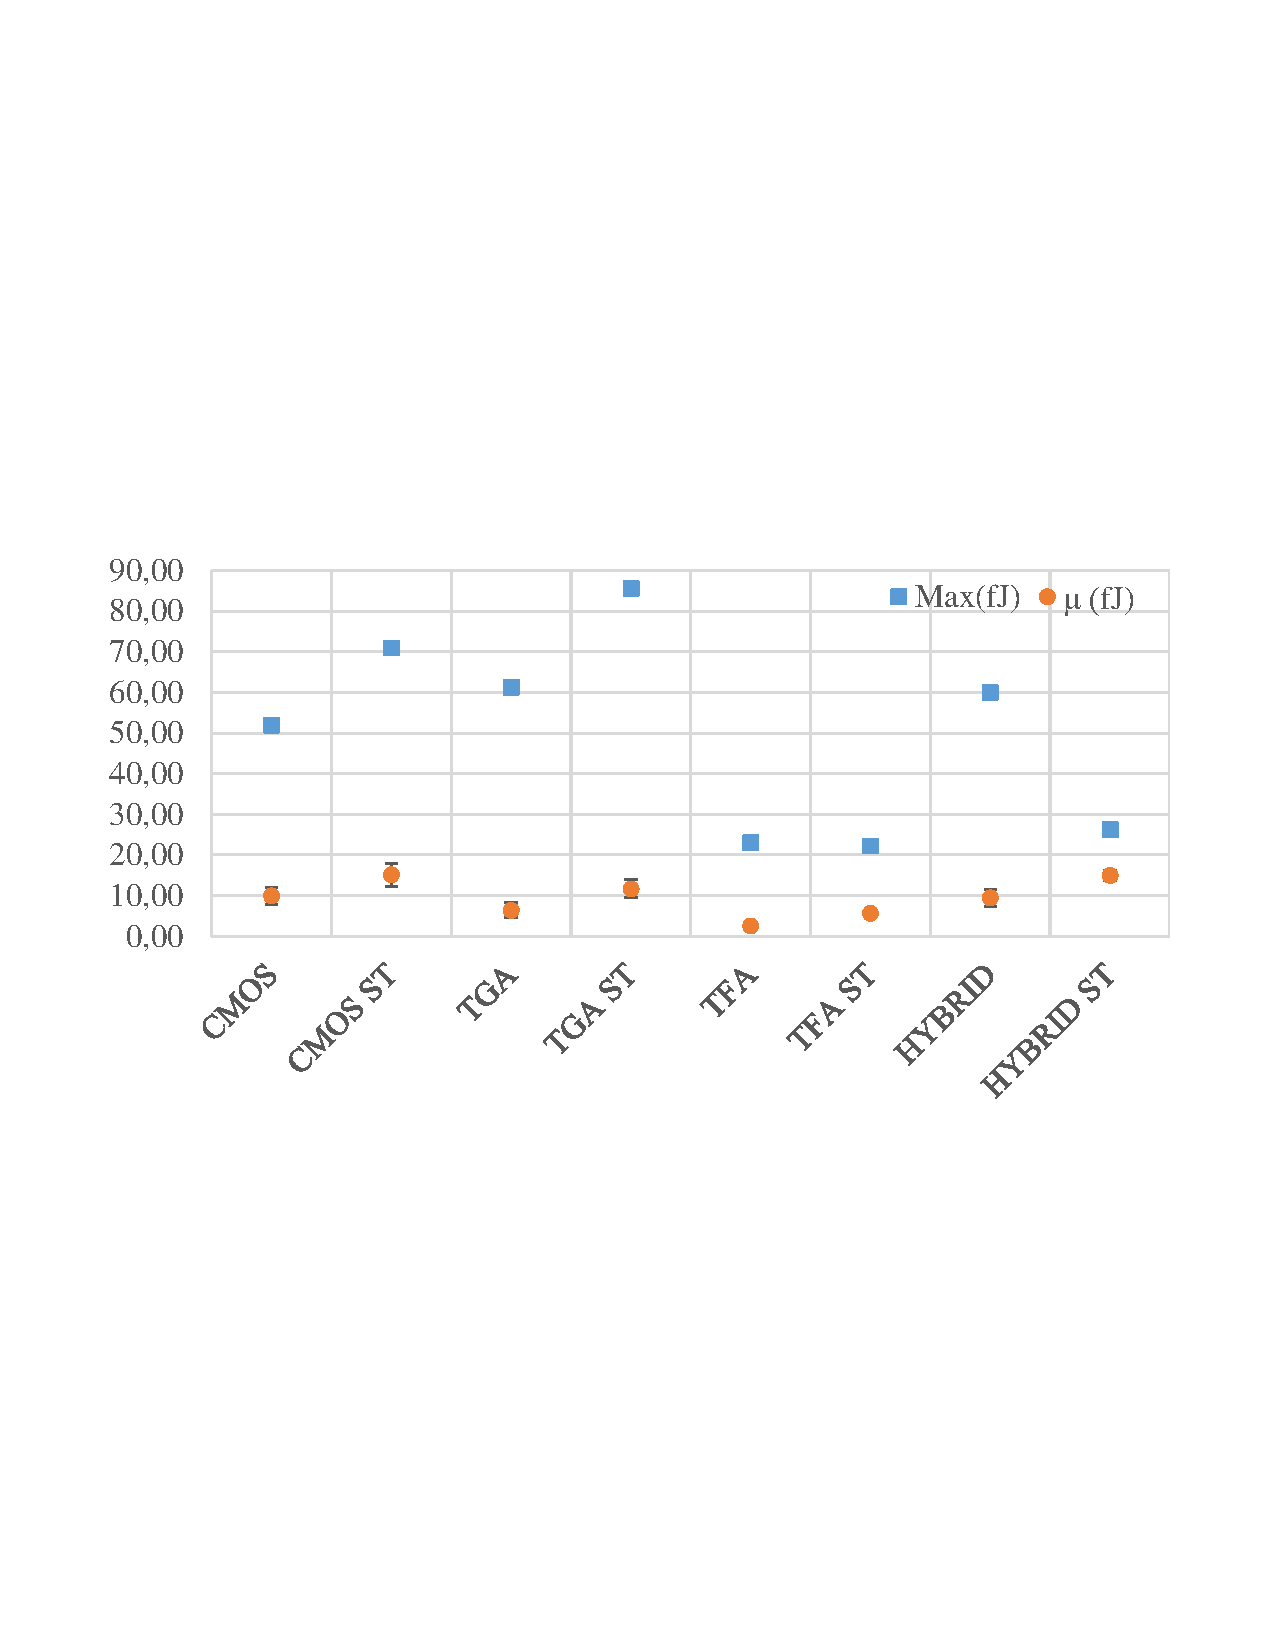
\includegraphics[width=\textwidth, trim={0 9cm 0 9cm},clip]{energyNTCarryOut.pdf}
\caption{Energy penalties for the Carry Out output at Near-Threshold operation.}
\label{fig:energyNTCO}
\legend{Source: from author.}
\end{figure}

For area penalties there was 136\%, 188\%, 100\% and 213\% increase for the CMOS, TGA, TFA and Hybrid Full Adders, respectively. Their respective areas are shown in Table \ref{penalties}. Such high area penalties are mainly due to technology rules such as the 108nm well-spacing and the necessity to use TAP-Cells to explicitly connect the transistors back-gates to specific parts of the circuits or the supply/ground making the ST cell more prominent than expected. The FA layouts are shown from Figure \ref{CMOS} to \ref{HYBRID}.

\begin{table}[H]
\centering
\caption{Full Adders areas and respective technique area impact.}
\label{penalties}
\begin{tabular}{lccc}
\hline
\textbf{Full Adder} & \multicolumn{1}{l}{\textbf{\# of Transistors}} & \textbf{Area (${\mu m}^2$)} & \textbf{Ratio}        \\ \hline
\textbf{CMOS}       & 28                                              & 0.32             & \multirow{2}{*}{2.36} \\ \cline{1-3}
\textbf{CMOS ST}    & 32                                              & 0.76             &                       \\ \hline
\textbf{TGA}        & 20                                              & 0.50             & \multirow{2}{*}{2.88} \\ \cline{1-3}
\textbf{TGA ST}     & 28                                              & 1.43             &                       \\ \hline
\textbf{TFA}        & 16                                              & 0.44             & \multirow{2}{*}{2.00} \\ \cline{1-3}
\textbf{TFA ST}     & 20                                              & 0.87             &                       \\ \hline
\textbf{HYBRID}     & 26                                              & 0.47             & \multirow{2}{*}{3.13} \\ \cline{1-3}
\textbf{HYBRID ST}  & 34                                              & 1.46             &                       \\ \hline
\end{tabular}
\end{table}

\begin{figure}[H]
  \centering
  \begin{subfigure}{\linewidth}
    \centering
    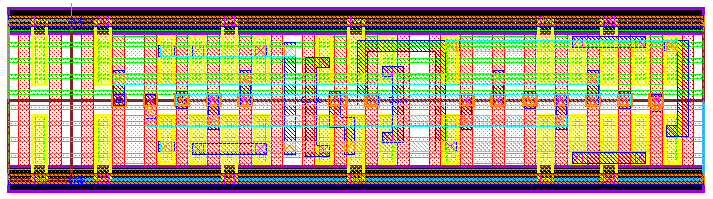
\includegraphics[width=\linewidth]{CMOS.png}
    \caption{Original Mirror CMOS Full Adder layout.}
  \end{subfigure}

  \begin{subfigure}{\linewidth}
    \centering
    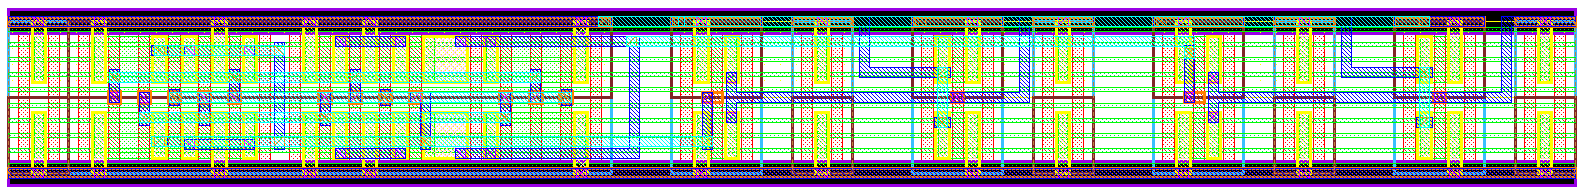
\includegraphics[width=\linewidth]{CMOSST.png}
    \caption{Mirror CMOS Full Adder layout with the applied technique.}
  \end{subfigure}  
  \caption{Mirror CMOS Full Adder layouts.}
 \label{CMOS}
\legend{Source: from author.}
\end{figure}

\begin{figure}[H]
  \centering
  \begin{subfigure}{\linewidth}
    \centering
    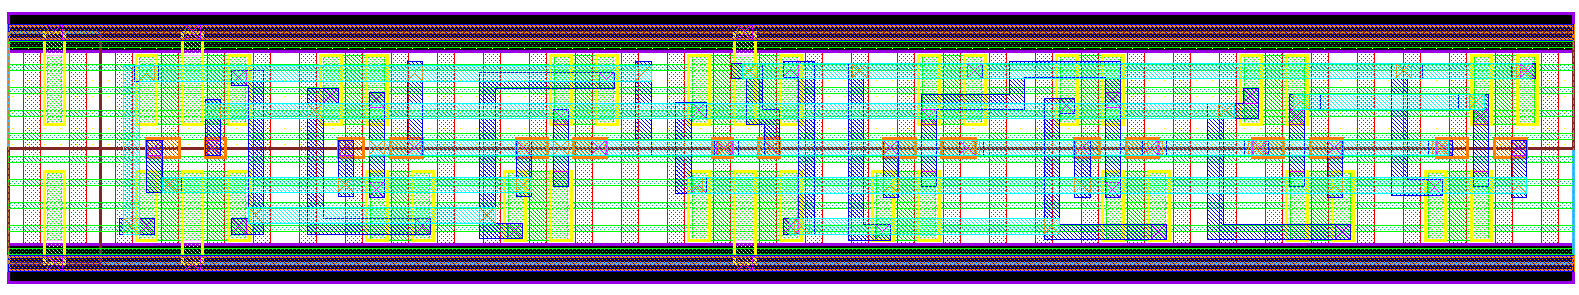
\includegraphics[width=\linewidth]{TGA.png}
    \caption{Original TGA Full Adder layout.}
  \end{subfigure}

  \begin{subfigure}{\linewidth}
    \centering
    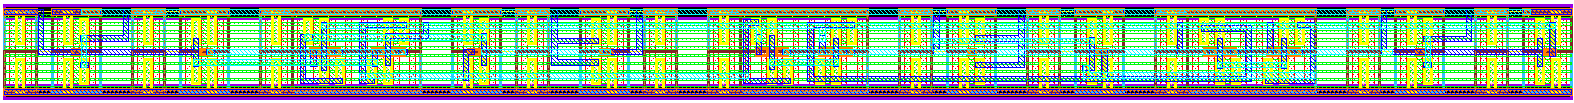
\includegraphics[width=\linewidth]{TGAST.png}
    \caption{TGA Full Adder layout with the applied technique.}
  \end{subfigure}  
  \caption{TGA Full Adder layouts.}
  \label{TGA}
\legend{Source: from author.}
\end{figure}

\begin{figure}[H]
  \centering
  \begin{subfigure}{\linewidth}
    \centering
    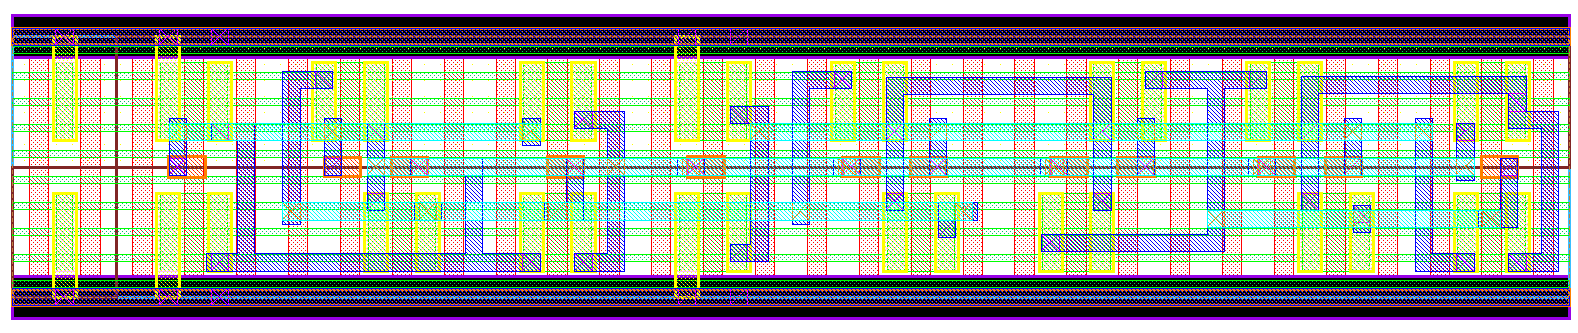
\includegraphics[width=\linewidth]{TFA.png}
    \caption{Original TFA Full Adder layout.}
  \end{subfigure}

  \begin{subfigure}{\linewidth}
    \centering
    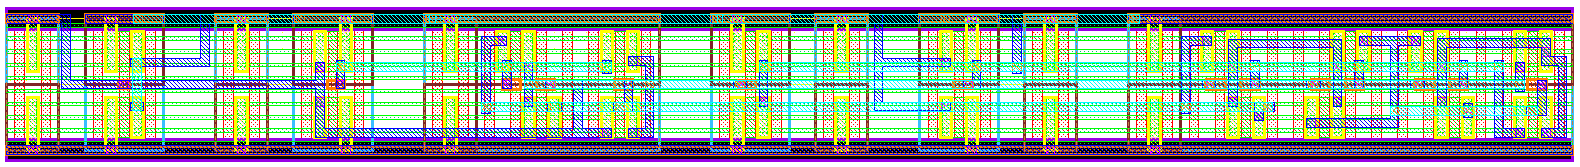
\includegraphics[width=\linewidth]{TFAST.png}
    \caption{TFA Full Adder layout with the applied technique.}
  \end{subfigure}  
  \caption{TFA Full Adder layouts.}
  \label{TFA}
\legend{Source: from author.}
\end{figure}

\begin{figure}[H]
  \centering
  \begin{subfigure}{\linewidth}
    \centering
    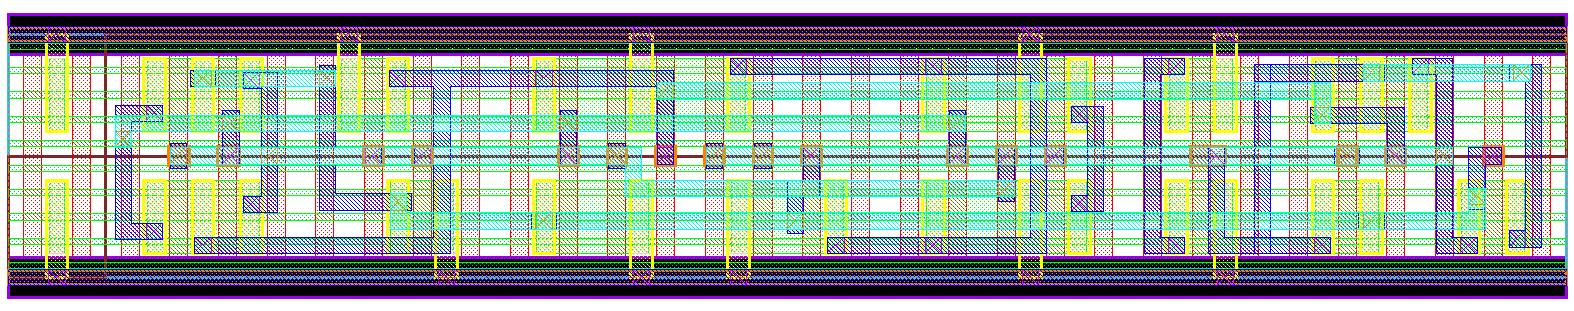
\includegraphics[width=\linewidth]{HYBRID.png}
    \caption{Original Hybrid Full Adder layout.}
  \end{subfigure}

  \begin{subfigure}{\linewidth}
    \centering
    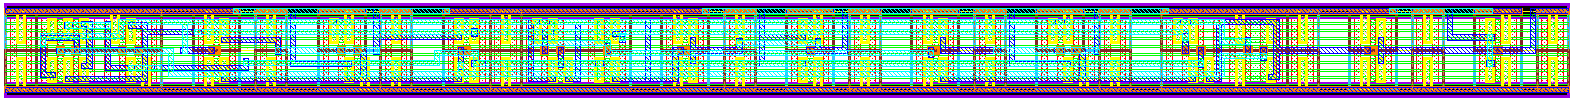
\includegraphics[width=\linewidth]{HYBRIDST.png}
    \caption{Hybrid Full Adder layout with the applied technique.}
  \end{subfigure}  
  \caption{Hybrid Full Adder layouts.}
  \label{HYBRID}
\legend{Source: from author.}
\end{figure}

\chapter{Conclusions}

Variability has been a critical challenge in emerging technology nodes because it can deviate from the correct circuit's behavior and affects the manufacturing yield. All current work in developing and validating techniques have been done at electrical and transistor level. There is a need for novel techniques which to improve variability robustness at the layout level.

Given that, a novel technique was tested. The method consists of replacing internal inverters with Schmitt Trigger inverters to increase the circuit’s noise-immunity. The ST technique presents considerable robustness improvements over all full adders. For nominal voltage and near-threshold operation, TFA and Hybrid adders showed the highest accumulated improvements, respectively. As results show, the technique improves, sometimes drastically, the energy variability robustness for each Full Adder considered. For delay robustness, in some cases, there was a worsening in robustness mainly caused by area penalty and the pass-transistor logic. 

Resuming, considering average variability robustness improvements with no worsenings, the Hybrid FA showed the best results for nominal voltage operation (17.64\%) and near-threshold operation (30.47\%). Considering only delay robustness there is no definitive best case at nominal voltage operation given that there was no considerable improvement at CMOS and Hybrid FAs and there was considerable worsening over one of the inputs at TGA and TFA. At near-threshold level the Hybrid FA brings the best average delay improvement (16.45\%). Considering only energy robustness improvements, the Hybrid FA showed the best average improvement (33.56\%) at nominal voltage operation. At near-threshold level, the TFA showed the best energy robustness improvement (61.88\%).

Considering penalties, the FA that suffered less penalty, at nominal voltage level, was the TGA, with 26\% increase on delays and 14\% increase in absolute delay deviations. At near-threshold level, the TFA showed improvements, with a 7\% decrease on delays and 17\% decrease on absolute deviations. Those improvements are due to the pass-transistor logic present on the TFA in a way that the extra path to supply/ground, comparing a inverter with the ST, aids the signal restoring. Alongside that, the TFA was the FA that presented the lowest area penalty. For energy penalties, the CMOS showed the lowest penalties, with 52\% increase in energy consumption and 24\% increase in absolute deviations. For near-threshold operation, the CMOS Adder shows again the lowest increase in energy consumption with the TFA showing a 10\% decrease in energy absolute deviation.

With the technique penalties in mind, it should only be utilized in applications that can bear the delays, energy consumption and area increase with variability robustness as a priority. These works demonstrate the need for new techniques at layout level to address variability for high performance/low power applications with low area penalties. It is important to note that, according to the state-of-art research, this is the first analysis of this technique made at layout level. For future works, a supply voltage calibration shall be made to find the best cost-benefit supply voltage.

\section{Future Works}

As future works it is proposed: a near-threshold voltage calibration to find the best cost-benefit supply voltage, to explore different full adder topologies and investigate other techniques to mitigate the impact of process variability.



\bibliographystyle{abntex2-alf}
\bibliography{biblio}
\annex
\chapter{Exemplo de arquivo utilizado na simulação elétrica sem a técnica ST}

\begin{lstlisting}
* test file for extracted cmos full adder layout with asap7 finfet tech
.include "CMOSFA.pex.netlist"
.include "/home/ic/leonardo.moraes/Desktop/FAEXT/hspice/7nm_TT.pm"

*.OPTION POST = 2
.define gauss(nom, rvar, sig) (nom + (nom*rvar)/sig * sgauss(0))

.param VCC = 0.7

.param p_phig = gauss(4.8108, 0.05, 3)
.param n_phig = gauss(4.3720, 0.05, 3)

VCIN CIN GND PWL (0n 0 18n 0)

VA1 A1 GND PWL (0n VCC 18n VCC)
VA2 A2 GND PWL (0n VCC 18n VCC)
VA4 A4 GND PWL (0n 0 18n 0)
VA5 A5 GND PWL (0n 0 18n 0)

VB2 B2 GND PWL (0n 0 18n 0)
VB4 B4 GND PWL (0n 0 18n 0)
VB5 B5 GND PWL (0n 0 18n 0)

VA3 A3 GND PWL (0n 0 3n 0 3.01n VCC 6n VCC 6.01n 0 7n 0 7.01n VCC 8n VCC 8.01n 0 10n 0 10.01n VCC 11n VCC 11.01n 0 15n 0 15.01n VCC 18n VCC)
VB3 B3 GND PWL (0n 0 3n 0 3.01n VCC 6n VCC 6.01n 0 9n 0 9.01n VCC 12n VCC 12.01n 0 13n 0 13.01n VCC 14n VCC 14.01n 0 16n 0 16.01n VCC 17n VCC 17.01n 0 18n 0)
VB1 B1 GND PWL (0n 0 1n 0 1.01n VCC 2n VCC 2.01n 0 3n 0 4n 0 4.01n VCC 5n VCC 5.01n 0 6n 0 9n 0 9.01n VCC 10n VCC 12n VCC 12.01n 0 13n 0 15n 0 15.01n VCC 16n VCC 18n VCC)

VVDD0 VDD0 GND VCC
VVDD1 VDD1 GND VCC
VGND GND GND 0

XCMOSFA1 GND VDD0 B1 A1 CIN   COUT1 SUM1 CMOSFA
XCMOSFA2 GND VDD0 B2 A2 COUT1 COUT2 SUM2 CMOSFA
XCMOSFA3 GND VDD1 B3 A3 COUT2 COUT3 SUM3 CMOSFA
XCMOSFA4 GND VDD0 B4 A4 COUT3 COUT4 SUM4 CMOSFA
XCMOSFA5 GND VDD0 B5 A5 COUT4 COUT5 SUM5 CMOSFA


.tran 1p 18n sweep Monte = 2000

    
    *---Atrasos de Propagacao----
    .measure tran TP_LH_Cin_0_1 trig v(COUT2) val=0.35 rise=1 targ v(SUM3) val=0.35 rise=1
    .measure tran TP_HL_Cin_0_1 trig v(COUT2) val=0.35 fall=1 targ v(SUM3) val=0.35 fall=1
    .measure tran TP_LH_Cin_1_0 trig v(COUT2) val=0.35 rise=2 targ v(SUM3) val=0.35 rise=2
    .measure tran TP_HL_Cin_1_0 trig v(COUT2) val=0.35 fall=2 targ v(SUM3) val=0.35 fall=2

    .measure tran TP_LH_0_A_1 trig v(A3) val=0.35 rise=2 targ v(SUM3) val=0.35 rise=3
    .measure tran TP_HL_0_A_1 trig v(A3) val=0.35 fall=2 targ v(SUM3) val=0.35 fall=3
    .measure tran TP_LH_1_A_0 trig v(A3) val=0.35 rise=3 targ v(SUM3) val=0.35 rise=5
    .measure tran TP_HL_1_A_0 trig v(A3) val=0.35 fall=3 targ v(SUM3) val=0.35 fall=5

    .measure tran TP_LH_0_1_B trig v(B3) val=0.35 rise=3 targ v(SUM3) val=0.35 rise=7
    .measure tran TP_HL_0_1_B trig v(B3) val=0.35 fall=3 targ v(SUM3) val=0.35 fall=7
    .measure tran TP_LH_1_0_B trig v(B3) val=0.35 rise=4 targ v(SUM3) val=0.35 rise=9
    .measure tran TP_HL_1_0_B trig v(B3) val=0.35 fall=4 targ v(SUM3) val=0.35 fall=9   
    
    *---Medidas de energia---
    .measure tran energy integ i(VVDD1) from=0n to=18n
    
.end
\end{lstlisting}

\chapter{Exemplo de arquivo utilizado na simulação elétrica com a técnica ST}

\begin{lstlisting}
* test file for extracted cmos full adder layout with asap7 finfet tech
.include "CMOSFAST.pex.netlist"
.include "/home/ic/leonardo.moraes/Desktop/FAEXT/hspice/7nm_TT.pm"

*.OPTION POST = 2
.define gauss(nom, rvar, sig) (nom + (nom*rvar)/sig * sgauss(0))

.param VCC = 0.7

.param p_phig = gauss(4.8108, 0.05, 3)
.param n_phig = gauss(4.3720, 0.05, 3)

VCIN CIN GND PWL (0n 0 18n 0)

VA1 A1 GND PWL (0n VCC 18n VCC)
VA2 A2 GND PWL (0n VCC 18n VCC)
VA4 A4 GND PWL (0n 0 18n 0)
VA5 A5 GND PWL (0n 0 18n 0)

VB2 B2 GND PWL (0n 0 18n 0)
VB4 B4 GND PWL (0n 0 18n 0)
VB5 B5 GND PWL (0n 0 18n 0)

VA3 A3 GND PWL (0n 0 3n 0 3.01n VCC 6n VCC 6.01n 0 7n 0 7.01n VCC 8n VCC 8.01n 0 10n 0 10.01n VCC 11n VCC 11.01n 0 15n 0 15.01n VCC 18n VCC)
VB3 B3 GND PWL (0n 0 3n 0 3.01n VCC 6n VCC 6.01n 0 9n 0 9.01n VCC 12n VCC 12.01n 0 13n 0 13.01n VCC 14n VCC 14.01n 0 16n 0 16.01n VCC 17n VCC 17.01n 0 18n 0)
VB1 B1 GND PWL (0n 0 1n 0 1.01n VCC 2n VCC 2.01n 0 3n 0 4n 0 4.01n VCC 5n VCC 5.01n 0 6n 0 9n 0 9.01n VCC 10n VCC 12n VCC 12.01n 0 13n 0 15n 0 15.01n VCC 16n VCC 18n VCC)

VVDD0 VDD0 GND VCC
VVDD1 VDD1 GND VCC
VGND GND GND 0

XCMOSFAST1 GND VDD0 B1 A1 CIN   COUT1 SUM1 CMOSFAST
XCMOSFAST2 GND VDD0 B2 A2 COUT1 COUT2 SUM2 CMOSFAST
XCMOSFAST3 GND VDD1 B3 A3 COUT2 COUT3 SUM3 CMOSFAST
XCMOSFAST4 GND VDD0 B4 A4 COUT3 COUT4 SUM4 CMOSFAST
XCMOSFAST5 GND VDD0 B5 A5 COUT4 COUT5 SUM5 CMOSFAST


.tran 1p 18n sweep Monte = 2000

    
    *---Atrasos de Propagacao----
    .measure tran TP_LH_Cin_0_1 trig v(COUT2) val=0.35 rise=1 targ v(SUM3) val=0.35 rise=1

    .measure tran TP_HL_Cin_0_1 trig v(COUT2) val=0.35 fall=1 targ v(SUM3) val=0.35 fall=1

    .measure tran TP_LH_Cin_1_0 trig v(COUT2) val=0.35 rise=2 targ v(SUM3) val=0.35 rise=2

    .measure tran TP_HL_Cin_1_0 trig v(COUT2) val=0.35 fall=2 targ v(SUM3) val=0.35 fall=2

    .measure tran TP_LH_0_A_1 trig v(A3) val=0.35 rise=2 targ v(SUM3) val=0.35 rise=3

    .measure tran TP_HL_0_A_1 trig v(A3) val=0.35 fall=2 targ v(SUM3) val=0.35 fall=3

    .measure tran TP_LH_1_A_0 trig v(A3) val=0.35 rise=3 targ v(SUM3) val=0.35 rise=5

    .measure tran TP_HL_1_A_0 trig v(A3) val=0.35 fall=3 targ v(SUM3) val=0.35 fall=5


    .measure tran TP_LH_0_1_B trig v(B3) val=0.35 rise=3 targ v(SUM3) val=0.35 rise=7

    .measure tran TP_HL_0_1_B trig v(B3) val=0.35 fall=3 targ v(SUM3) val=0.35 fall=7

    .measure tran TP_LH_1_0_B trig v(B3) val=0.35 rise=4 targ v(SUM3) val=0.35 rise=9

    .measure tran TP_HL_1_0_B trig v(B3) val=0.35 fall=4 targ v(SUM3) val=0.35 fall=9   
    
    *---Medidas de energia---
    .measure tran energy integ i(VVDD1) from=0n to=18n
    
.end
\end{lstlisting}

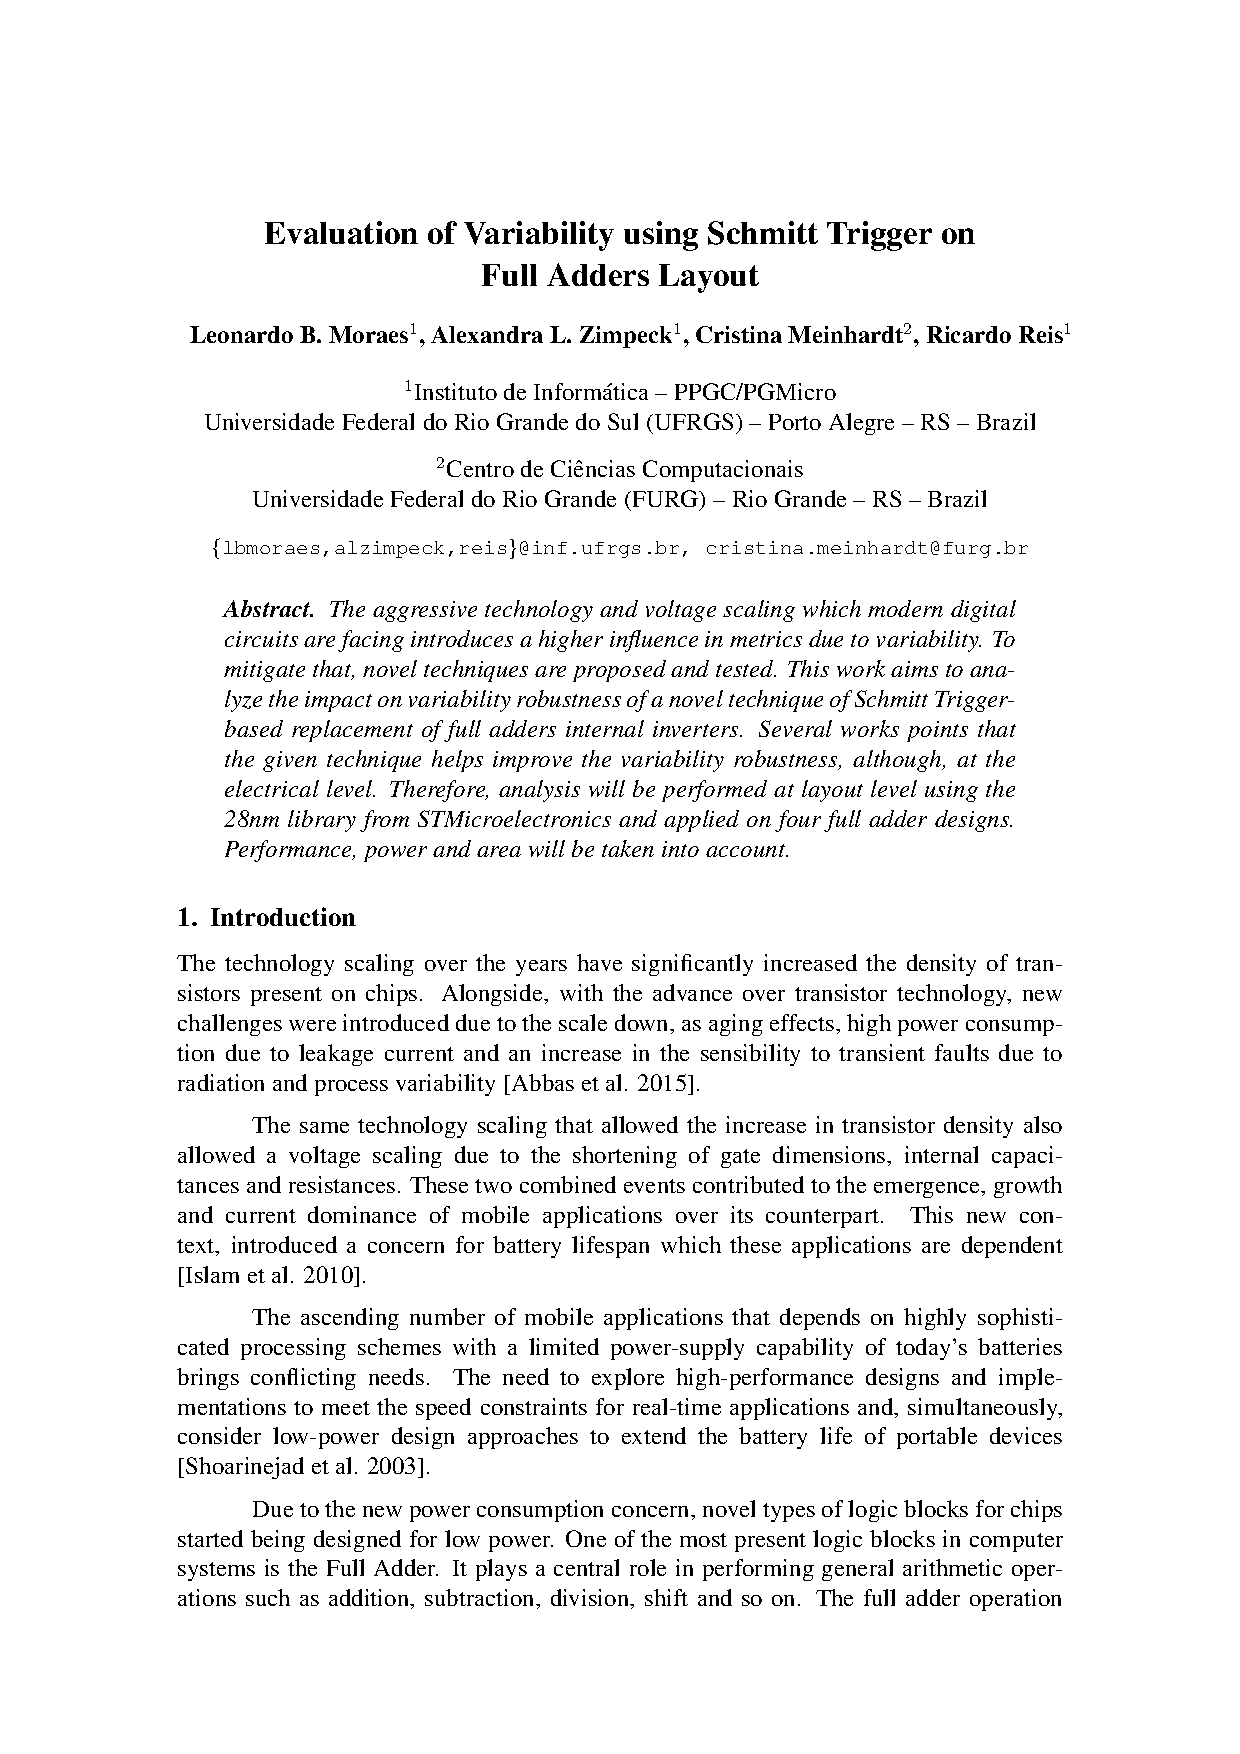
\includepdf[pages=-]{TG1.pdf}
\end{document}